% Options for packages loaded elsewhere
\PassOptionsToPackage{unicode}{hyperref}
\PassOptionsToPackage{hyphens}{url}
%
\documentclass[
  12pt,
]{book}
\usepackage{amsmath,amssymb}
\usepackage{iftex}
\ifPDFTeX
  \usepackage[T1]{fontenc}
  \usepackage[utf8]{inputenc}
  \usepackage{textcomp} % provide euro and other symbols
\else % if luatex or xetex
  \usepackage{unicode-math} % this also loads fontspec
  \defaultfontfeatures{Scale=MatchLowercase}
  \defaultfontfeatures[\rmfamily]{Ligatures=TeX,Scale=1}
\fi
\usepackage{lmodern}
\ifPDFTeX\else
  % xetex/luatex font selection
\fi
% Use upquote if available, for straight quotes in verbatim environments
\IfFileExists{upquote.sty}{\usepackage{upquote}}{}
\IfFileExists{microtype.sty}{% use microtype if available
  \usepackage[]{microtype}
  \UseMicrotypeSet[protrusion]{basicmath} % disable protrusion for tt fonts
}{}
\makeatletter
\@ifundefined{KOMAClassName}{% if non-KOMA class
  \IfFileExists{parskip.sty}{%
    \usepackage{parskip}
  }{% else
    \setlength{\parindent}{0pt}
    \setlength{\parskip}{6pt plus 2pt minus 1pt}}
}{% if KOMA class
  \KOMAoptions{parskip=half}}
\makeatother
\usepackage{xcolor}
\usepackage{color}
\usepackage{fancyvrb}
\newcommand{\VerbBar}{|}
\newcommand{\VERB}{\Verb[commandchars=\\\{\}]}
\DefineVerbatimEnvironment{Highlighting}{Verbatim}{commandchars=\\\{\}}
% Add ',fontsize=\small' for more characters per line
\usepackage{framed}
\definecolor{shadecolor}{RGB}{248,248,248}
\newenvironment{Shaded}{\begin{snugshade}}{\end{snugshade}}
\newcommand{\AlertTok}[1]{\textcolor[rgb]{0.94,0.16,0.16}{#1}}
\newcommand{\AnnotationTok}[1]{\textcolor[rgb]{0.56,0.35,0.01}{\textbf{\textit{#1}}}}
\newcommand{\AttributeTok}[1]{\textcolor[rgb]{0.13,0.29,0.53}{#1}}
\newcommand{\BaseNTok}[1]{\textcolor[rgb]{0.00,0.00,0.81}{#1}}
\newcommand{\BuiltInTok}[1]{#1}
\newcommand{\CharTok}[1]{\textcolor[rgb]{0.31,0.60,0.02}{#1}}
\newcommand{\CommentTok}[1]{\textcolor[rgb]{0.56,0.35,0.01}{\textit{#1}}}
\newcommand{\CommentVarTok}[1]{\textcolor[rgb]{0.56,0.35,0.01}{\textbf{\textit{#1}}}}
\newcommand{\ConstantTok}[1]{\textcolor[rgb]{0.56,0.35,0.01}{#1}}
\newcommand{\ControlFlowTok}[1]{\textcolor[rgb]{0.13,0.29,0.53}{\textbf{#1}}}
\newcommand{\DataTypeTok}[1]{\textcolor[rgb]{0.13,0.29,0.53}{#1}}
\newcommand{\DecValTok}[1]{\textcolor[rgb]{0.00,0.00,0.81}{#1}}
\newcommand{\DocumentationTok}[1]{\textcolor[rgb]{0.56,0.35,0.01}{\textbf{\textit{#1}}}}
\newcommand{\ErrorTok}[1]{\textcolor[rgb]{0.64,0.00,0.00}{\textbf{#1}}}
\newcommand{\ExtensionTok}[1]{#1}
\newcommand{\FloatTok}[1]{\textcolor[rgb]{0.00,0.00,0.81}{#1}}
\newcommand{\FunctionTok}[1]{\textcolor[rgb]{0.13,0.29,0.53}{\textbf{#1}}}
\newcommand{\ImportTok}[1]{#1}
\newcommand{\InformationTok}[1]{\textcolor[rgb]{0.56,0.35,0.01}{\textbf{\textit{#1}}}}
\newcommand{\KeywordTok}[1]{\textcolor[rgb]{0.13,0.29,0.53}{\textbf{#1}}}
\newcommand{\NormalTok}[1]{#1}
\newcommand{\OperatorTok}[1]{\textcolor[rgb]{0.81,0.36,0.00}{\textbf{#1}}}
\newcommand{\OtherTok}[1]{\textcolor[rgb]{0.56,0.35,0.01}{#1}}
\newcommand{\PreprocessorTok}[1]{\textcolor[rgb]{0.56,0.35,0.01}{\textit{#1}}}
\newcommand{\RegionMarkerTok}[1]{#1}
\newcommand{\SpecialCharTok}[1]{\textcolor[rgb]{0.81,0.36,0.00}{\textbf{#1}}}
\newcommand{\SpecialStringTok}[1]{\textcolor[rgb]{0.31,0.60,0.02}{#1}}
\newcommand{\StringTok}[1]{\textcolor[rgb]{0.31,0.60,0.02}{#1}}
\newcommand{\VariableTok}[1]{\textcolor[rgb]{0.00,0.00,0.00}{#1}}
\newcommand{\VerbatimStringTok}[1]{\textcolor[rgb]{0.31,0.60,0.02}{#1}}
\newcommand{\WarningTok}[1]{\textcolor[rgb]{0.56,0.35,0.01}{\textbf{\textit{#1}}}}
\usepackage{longtable,booktabs,array}
\usepackage{calc} % for calculating minipage widths
% Correct order of tables after \paragraph or \subparagraph
\usepackage{etoolbox}
\makeatletter
\patchcmd\longtable{\par}{\if@noskipsec\mbox{}\fi\par}{}{}
\makeatother
% Allow footnotes in longtable head/foot
\IfFileExists{footnotehyper.sty}{\usepackage{footnotehyper}}{\usepackage{footnote}}
\makesavenoteenv{longtable}
\usepackage{graphicx}
\makeatletter
\def\maxwidth{\ifdim\Gin@nat@width>\linewidth\linewidth\else\Gin@nat@width\fi}
\def\maxheight{\ifdim\Gin@nat@height>\textheight\textheight\else\Gin@nat@height\fi}
\makeatother
% Scale images if necessary, so that they will not overflow the page
% margins by default, and it is still possible to overwrite the defaults
% using explicit options in \includegraphics[width, height, ...]{}
\setkeys{Gin}{width=\maxwidth,height=\maxheight,keepaspectratio}
% Set default figure placement to htbp
\makeatletter
\def\fps@figure{htbp}
\makeatother
\setlength{\emergencystretch}{3em} % prevent overfull lines
\providecommand{\tightlist}{%
  \setlength{\itemsep}{0pt}\setlength{\parskip}{0pt}}
\setcounter{secnumdepth}{5}
\usepackage{booktabs}
\ifLuaTeX
  \usepackage{selnolig}  % disable illegal ligatures
\fi
\usepackage[]{natbib}
\bibliographystyle{apalike}
\IfFileExists{bookmark.sty}{\usepackage{bookmark}}{\usepackage{hyperref}}
\IfFileExists{xurl.sty}{\usepackage{xurl}}{} % add URL line breaks if available
\urlstyle{same}
\hypersetup{
  pdftitle={Introduction to Term Structure Models},
  pdfauthor={Jean-Paul Renne and Alain Monfort},
  hidelinks,
  pdfcreator={LaTeX via pandoc}}

\title{Introduction to Term Structure Models}
\author{Jean-Paul Renne and Alain Monfort}
\date{2024-01-26}

\usepackage{amsthm}
\newtheorem{theorem}{Theorem}[chapter]
\newtheorem{lemma}{Lemma}[chapter]
\newtheorem{corollary}{Corollary}[chapter]
\newtheorem{proposition}{Proposition}[chapter]
\newtheorem{conjecture}{Conjecture}[chapter]
\theoremstyle{definition}
\newtheorem{definition}{Definition}[chapter]
\theoremstyle{definition}
\newtheorem{example}{Example}[chapter]
\theoremstyle{definition}
\newtheorem{exercise}{Exercise}[chapter]
\theoremstyle{definition}
\newtheorem{hypothesis}{Hypothesis}[chapter]
\theoremstyle{remark}
\newtheorem*{remark}{Remark}
\newtheorem*{solution}{Solution}
\begin{document}
\maketitle

{
\setcounter{tocdepth}{1}
\tableofcontents
}
\newcommand{\bv}[1]{\mathbf{#1}}

\hypertarget{intro}{%
\chapter*{Introduction to Term Structure Models}\label{intro}}

Modeling dynamic term structures serves as a practical and indispensable tool in the realm of finance. It enables investors, institutions, and policymakers to make informed decisions, manage risk effectively, and allocate resources wisely. By understanding how interest rates and yields evolve over time, these models offer a clear lens through which to assess market trends and price financial instruments accurately.

This course has been developed by \href{https://sites.google.com/site/jeanpaulrenne/home}{Jean-Paul Renne} and \href{https://faculty.crest.fr/amonfort/}{Alain Monfort}. It is illustrated by R codes using various packages that can be obtained from \href{https://cran.r-project.org}{CRAN}. This \texttt{TSModels} package is available on GitHub. To install it, one need to employ the \texttt{devtools} library:

\begin{Shaded}
\begin{Highlighting}[]
\FunctionTok{install.packages}\NormalTok{(}\StringTok{"devtools"}\NormalTok{) }\CommentTok{\# in case this library has not been loaded yet}
\FunctionTok{library}\NormalTok{(devtools)}
\FunctionTok{install\_github}\NormalTok{(}\StringTok{"jrenne/TSModels"}\NormalTok{)}
\FunctionTok{library}\NormalTok{(AEC)}
\end{Highlighting}
\end{Shaded}

\textbf{Useful (R) links:}

\begin{itemize}
\item
  Download R:

  \begin{itemize}
  \tightlist
  \item
    R software: \url{https://cran.r-project.org} (the basic R software)
  \item
    RStudio: \url{https://www.rstudio.com} (a convenient R editor)
  \end{itemize}
\item
  Tutorials:

  \begin{itemize}
  \tightlist
  \item
    Rstudio: \url{https://dss.princeton.edu/training/RStudio101.pdf} (by Oscar Torres-Reyna)
  \item
    R: \url{https://cran.r-project.org/doc/contrib/Paradis-rdebuts_en.pdf} (by Emmanuel Paradis)
  \item
    My own tutorial: \url{https://jrenne.shinyapps.io/Rtuto_publiShiny/}
  \end{itemize}
\end{itemize}

\hypertarget{Structural}{%
\chapter{A detour through structural approaches}\label{Structural}}

\hypertarget{basics-of-structural-approaches-c-capm}{%
\section{Basics of Structural Approaches: C-CAPM}\label{basics-of-structural-approaches-c-capm}}

\emph{Structural models} link the stochastic discount factor (SDF) to investor behavior through assumptions about preferences. Investors make portfolio decisions to obtain a desired time and risk profile of consumption. Loosely speaking, the SDF \(\mathcal{M}_{t,t+1}\) captures the aspects of utility that matter for valuing the assets. A seminal example is that of the consumption capital asset pricing model, or CCAPM (see, e.g., \citet{Merton_1973} and \citet{BREEDEN1979265}). The CCAPM extends the CAPM framework by providing a consumption-based theory of the determinants of the valuation of the market portfolio.

In the basic CCAPM version, a representative investor with time-additive preferences operates in a complete market. It has been extended in several directions to account for more complex investor preferences (e.g., Epstein-Zin see XXX), investor heterogeneity, incomplete markets, borrowing restrictions.

Consider a representative agent maximizing her expected utility:
\[
U_t = \mathbb{E}_t \left[ \sum_{j=0}^\infty \delta^j u(C_{t+j}) \right],
\]
where \(u\) is a utility function of consumption and \(\delta\) is the subjective time discount factor (\(\ne\) SDF). The budget constraint of the agent is
\[
C_t + \sum_i w_{i,t} P_{i,t} \le \sum_i w_{i,t-1}\underbrace{(P_{i,t}+D_{i,t})}_{x_{i,t}} + Y_t,
\]
where \(Y_t\) is her labor income at date \(t\). The first-order condition (FOC) for intertemporal utility optimization yields, for asset \(i\):\footnote{This FOC states that the agent indifferent between investing an additional infinitesimal amount of asset \(i\) or not.}
\begin{equation}
P_{i,t} = \mathbb{E}_t \left[ \delta \frac{u'(C_{t+1})}{u'(C_{t})} x_{i,t+1} \right] = \mathbb{E}_t \left[ \mathcal{M}_{t,t+1} x_{i,t+1} \right],\label{eq:pricingcapm}
\end{equation}
where \(\mathcal{M}_{t,t+1}\) is the stochastic discount factor:
\[
\boxed{\mathcal{M}_{t,t+1}=\delta \dfrac{u'(C_{t+1})}{u'(C_{t})}.}
\]
Since \(u'\) is a decreasing function, the lower \(C_{t+1}\), the higher the SDF. Formula @ref(eq:pricingcapm\} implies that those assets whose payoffs are high during recessions (low \(C_{t+1}\)) are more expensive. As \citet{Cochrane_2005} puts it, the SDF can be seen as a measure of hunger: ``Good'' assets pay off well in bad times, when investors are hungry. Investors all want them, which drive up their price, and thereby lower their average returns.

The CCAPM is a simple model; it is easy to test once a form for \(u\) has been posited. It turns out it is difficult to reconcile with the data. In particular:

\begin{itemize}
\tightlist
\item
  Fitting average excess return implies implausible risk aversions (\emph{equity puzzle}).
\item
  The resulting risk-free short-term rate is too large unless risk aversion is small (\emph{interest-rate puzzle}).
\item
  It suggests maximum Sharpe ratios that are far too low \citep{Hansen_Jagannathan_1991}.
\end{itemize}

\begin{example}[Power utility function]
\protect\hypertarget{exm:powerU}{}\label{exm:powerU}

A power utility function is defined as follows:
\[
u(C_t) = \frac{C_t^{1-\gamma}}{1 - \gamma}.
\]
In that case \(\gamma\) has two interpretations:

\begin{itemize}
\tightlist
\item
  \emph{Relative Risk Aversion (RRA)} (see Definition \ref{def:RAmeasures}): aversion to variability \emph{across states of nature}.
\item
  \emph{Intertemporal Elasticity of Substitution} (see Definition \ref{def:IES}): aversion to variability \emph{across time}.
\end{itemize}

This is illustrated by Figure \ref{fig:RRAIESCCAPM}, that can concern two situations:

\begin{itemize}
\tightlist
\item
  Consider an agent whose consumption (on next period) can take two values \(C_l= 0.8\) or \(C_h= 1.2\), each with a probability of 0.5. Figure \ref{fig:RRAIESCCAPM} shows the associated \emph{expected} utility.
\item
  Consider a case with no uncertainty, and with \(\delta=1\). There are two periods: 0 and 1. One consumes \(C_l=0.8\) at date 0 and \(C_h=1.2\) at date 1. Figure \ref{fig:RRAIESCCAPM} shows the associated \emph{intertemporal} utility.
\end{itemize}

\begin{figure}
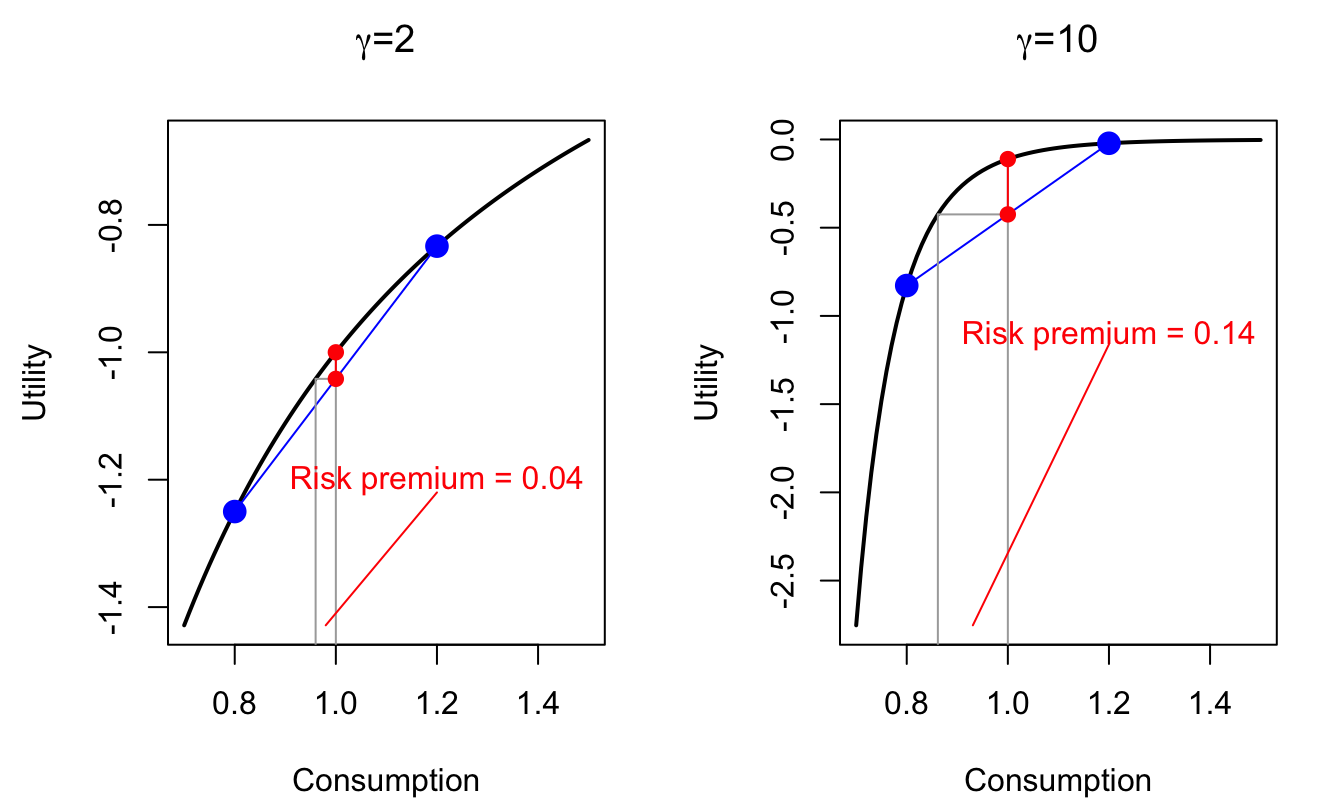
\includegraphics[width=0.95\linewidth]{TSM_files/figure-latex/RRAIESCCAPM-1} \caption{Power utility situation. Illustration of the RRA or the IES.}\label{fig:RRAIESCCAPM}
\end{figure}

\end{example}

\begin{definition}[Risk aversion measures]
\protect\hypertarget{def:RAmeasures}{}\label{def:RAmeasures}

Consider a utility function \(u\).

\begin{itemize}
\tightlist
\item
  The \emph{absolute risk aversion} is defined by:
  \[
  ARA = - \frac{u''(C)}{u'(C)}.
  \]
\item
  The \emph{relative risk aversion} is defined by:
  \[
  RRA = - \frac{C u''(C)}{u'(C)}.
  \]
  If \(u\) is concave, both measures are positive.
\end{itemize}

\end{definition}

\begin{definition}[Intertemporal Elasticity of Substitution]
\protect\hypertarget{def:IES}{}\label{def:IES}The \emph{Intertemporal Elasticity of Substitution (IES)} is defined as the change in consumption growth per change in the interest rate, that is:
\[
IES = \frac{d \log\left( \dfrac{C_{t+1}}{C_{t}}\right)}{d r} = - \frac{d \log\left( \dfrac{C_{t+1}}{C_{t}}\right)}{d\log\left(\dfrac{u'(C_{t+1})}{u'(C_{t})}\right)}.
\]
\end{definition}

Case of the isoelastic, or power, utility function. The isoelastic, or power, utility function defined by: \(u:\) \(C \rightarrow \dfrac{C^{1 - \gamma}-1}{1-\gamma}\) has a constant RRA of \(\gamma\).

Consider an agent whose wealth is \(W\). She can invest in an asset whose price is 1 and whose payoff is \(1+\varepsilon\) with probability \(1/2\) and \(1/(1+\varepsilon)\) with probability \(1/2\). Her utility function is denoted by \(u(.)\).

We want to compute the optimal share of wealth, denoted by \(\alpha\), invested in the asset. The expected utility is:
\[
\frac{1}{2}u\left(C(1-\alpha)+C\alpha(1+\varepsilon)\right) + \frac{1}{2}u\left(C(1-\alpha)+C\alpha/(1+\varepsilon)\right).
\]
Taking the second-order Taylor expansion of the previous expression and letting \(\varepsilon\) tend to zero, it appears that one has to maximize the following expression:
\[
\alpha u'(C) + \frac{1}{2}C \alpha^2 u''(C).
\]
Hence, the utility is maximized for:
\[
\alpha = - \frac{u'(C)}{C u''(C)} = \frac{1}{RRA}.
\]

Using Eq. \eqref{eq:MRCov}---that also applies in the present context---we get the following average excess return:
\begin{eqnarray*}
\mathbb{E}_t(R_{i,t+1} - R_{f,t}) &=& - (1 + R_{f,t}) \mathbb{C}ov_t\left(\delta \dfrac{u'(C_{t+1})}{u'(C_{t})},R_{i,t+1}\right)\\
&\approx& (1 + R_{f,t}) \delta \gamma  \mathbb{C}ov_t\left(\Delta c_{t+1},R_{i,t+1}\right),
\end{eqnarray*}
where \(\Delta c_{t+1} = \log(C_{t+1}/C_t)\).
Because consumption is smooth, the covariance \(\mathbb{C}ov_t\left(\Delta c_{t+1},R_{i,t+1}\right)\) is relatively small.
Hence, in order to replicate large average excess return, \(\gamma\) has to be big (see last two columns of the following table, from \citet{Campbell_1999}).

\begin{figure}

{\centering 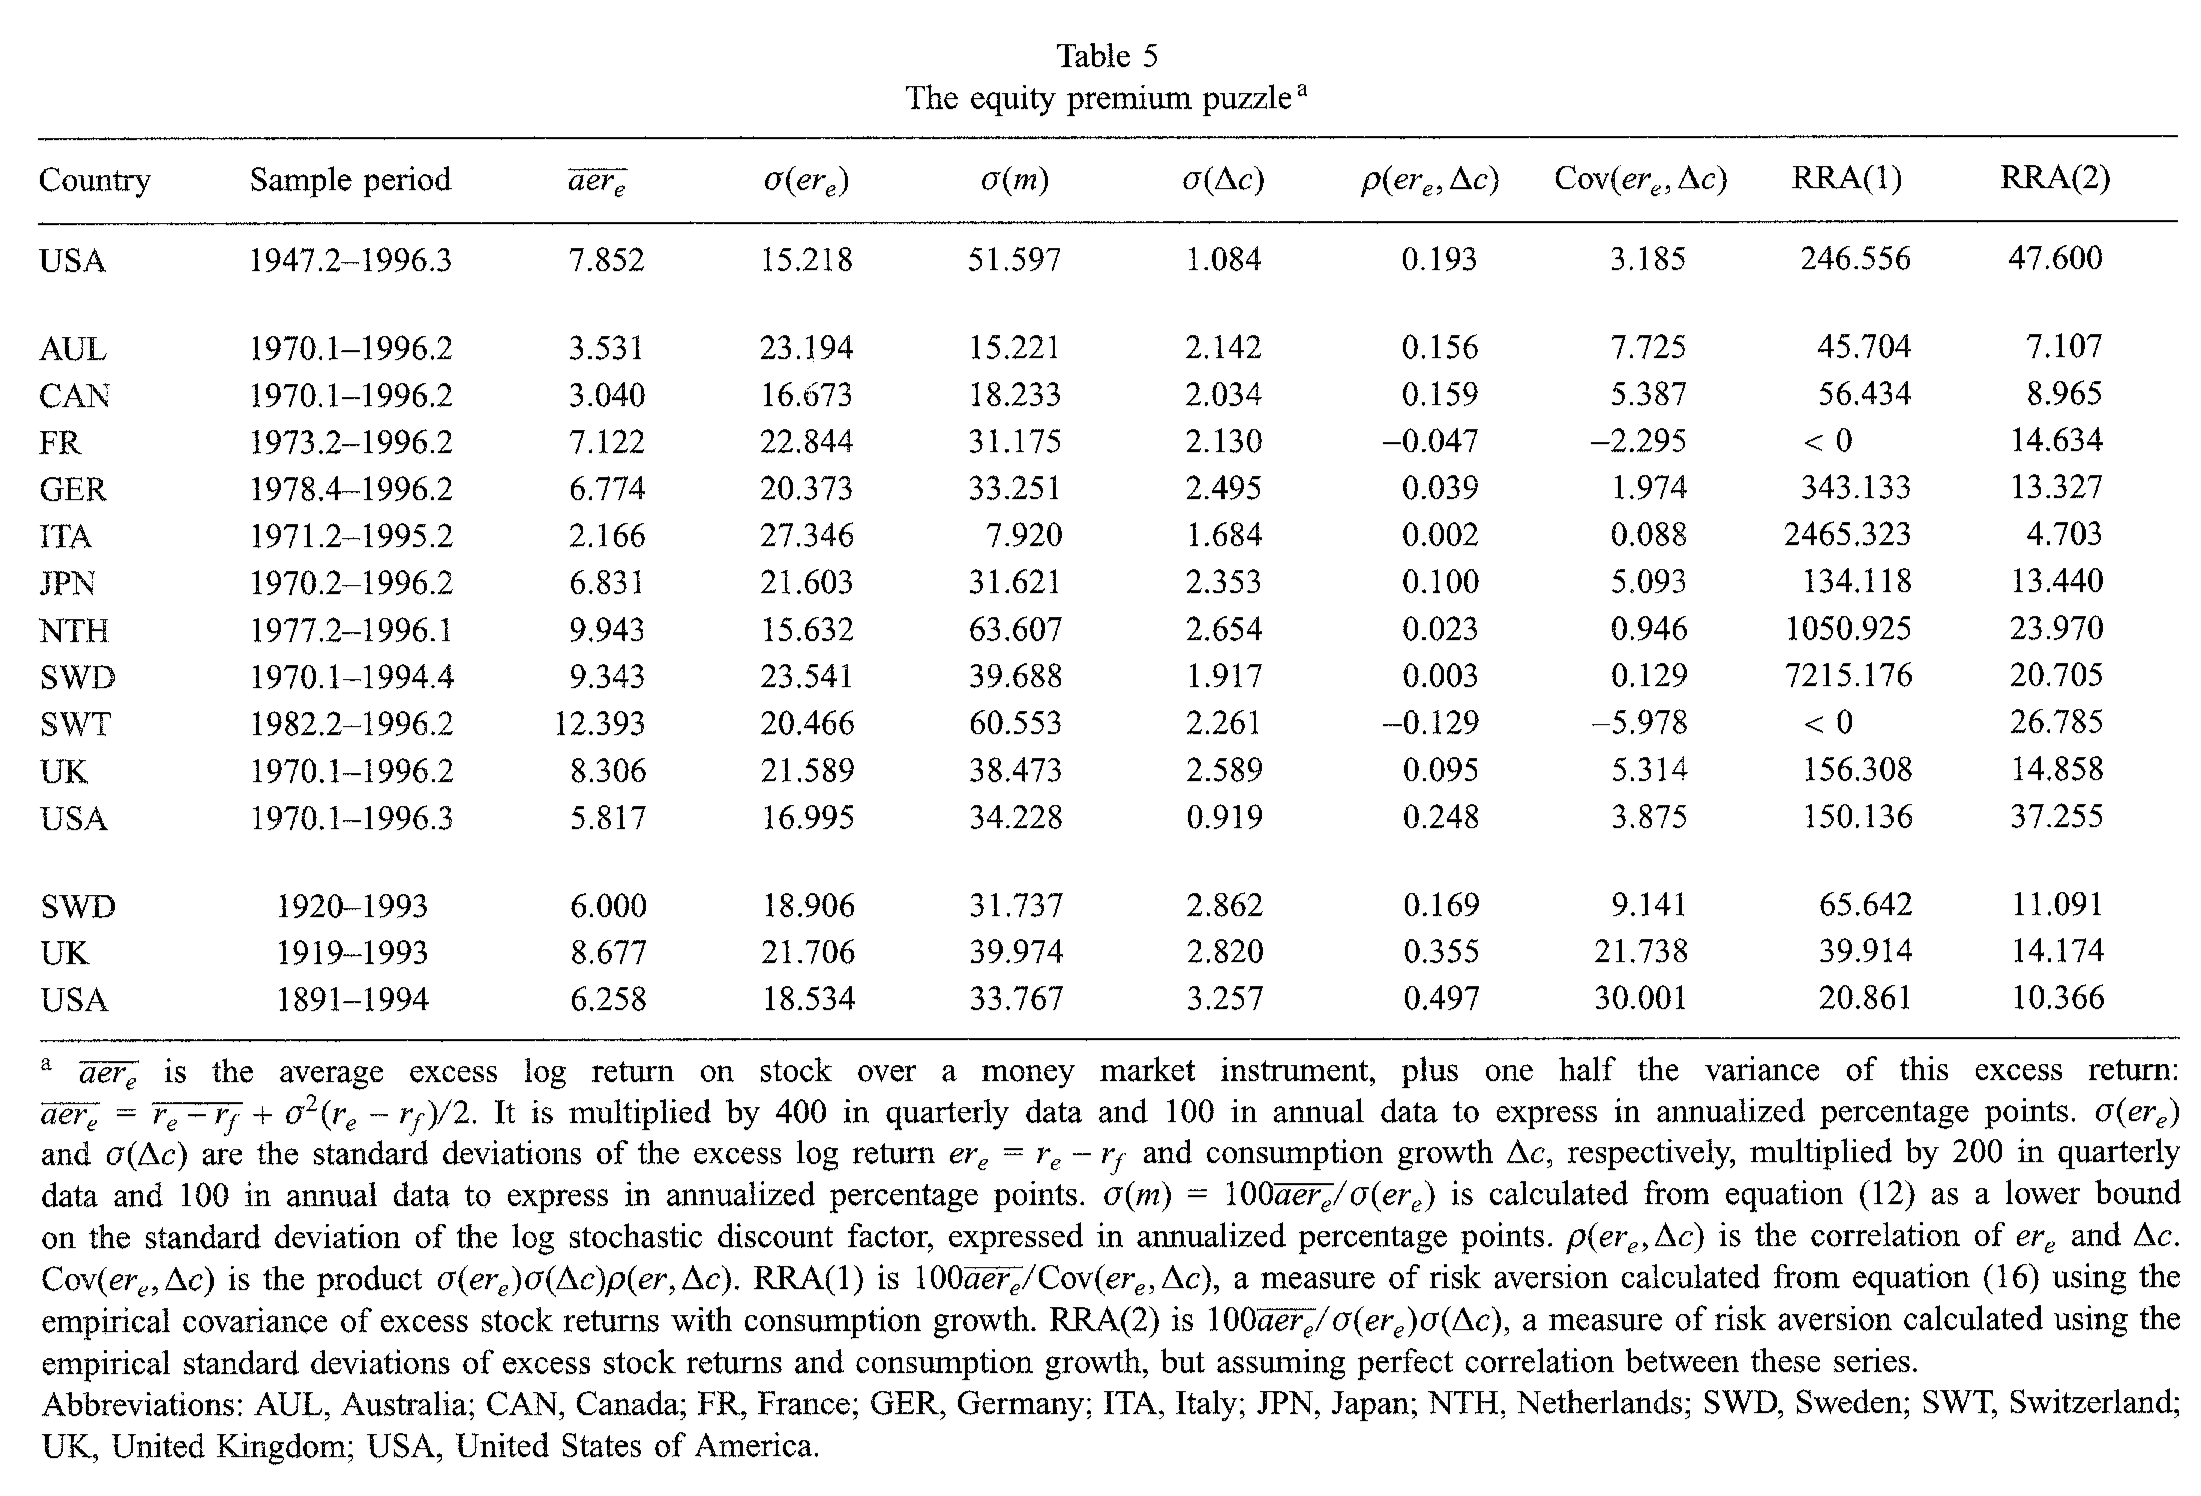
\includegraphics[width=1\linewidth]{figures/table_campbell1999_eqpuzzle} 

}

\caption{Source: Campbell (1999).}\label{fig:Campbell1}
\end{figure}

For sake of comparison: microeconomic study points to estimates of \(\gamma\) in \([1,3]\) (e.g., \citet{Hartley_Lanot_Walker_2014}).
\textbf{Equity premium puzzle} put forward by \citet{Mehra_Prescott_1985}.
\citet{Kandel_Stambaugh_1991}: Maybe that risk aversion is very high indeed?
But then, another substantial problem arise: If people are very risk averse, they want to transfer consumption from high levels to low levels.
In order to allow for a 2\% average increase in \(C_t\), the model predicts that average short-term rate should be high (to prevent people from borrowing too much). Such high interest rates are at odds with the data.
\textbf{Risk-free rate puzzle}.

In the case of the power utility function, the risk aversion is the inverse of the Intertemporal Elasticity of Substitution (Def. \ref{def:IES}):
\[
\mbox{High risk aversion} \Leftrightarrow \mbox{Low IES}.
\]
For given values of the risk-free rates \(R_{f,t}\), a decrease in the IES (increase in \(\gamma\)) leads people to make consumption smoother (see Example \ref{exm:IESsmooth}).
\[
\frac{1}{1+R_{f,t}} \approx \mathbb{E}_t(\delta (1 - \gamma \Delta c_{t+1}))
\]
Hence, for the very large values of \(\gamma\) necessary to fit average equity excess returns, agents strongly want to smoothen consumption.
To reconcile a high risk aversion this with the observed low real interest rate observed on average, it must be that investors are infinitely patients (\emph{risk-free rate puzzle}):
If \(\gamma=10\), \(R_{f,t} \approx 0\%\) and \(\Delta c_{t+1} \approx 2\%\), then \(\delta \approx 1.25\), which is not reasonable.

\begin{example}[IES and smoothing behavior]
\protect\hypertarget{exm:IESsmoothing}{}\label{exm:IESsmoothing}

The agents have a wealth of 1 unit that they consume over two periods. If they consume \(C_1\) in period, they consume \((1+R)(1-C_1)\) in period 2. They feature power-utility time-separable preferences with \(\delta=1\) and \(R=5\%\).

The optimization of the intertemporal utility of the agents imply that \(1/(1+R)=(C_2/C_1)^{-\gamma}\). Hence, the lower the IES, the smoother the consumption path.

\begin{figure}
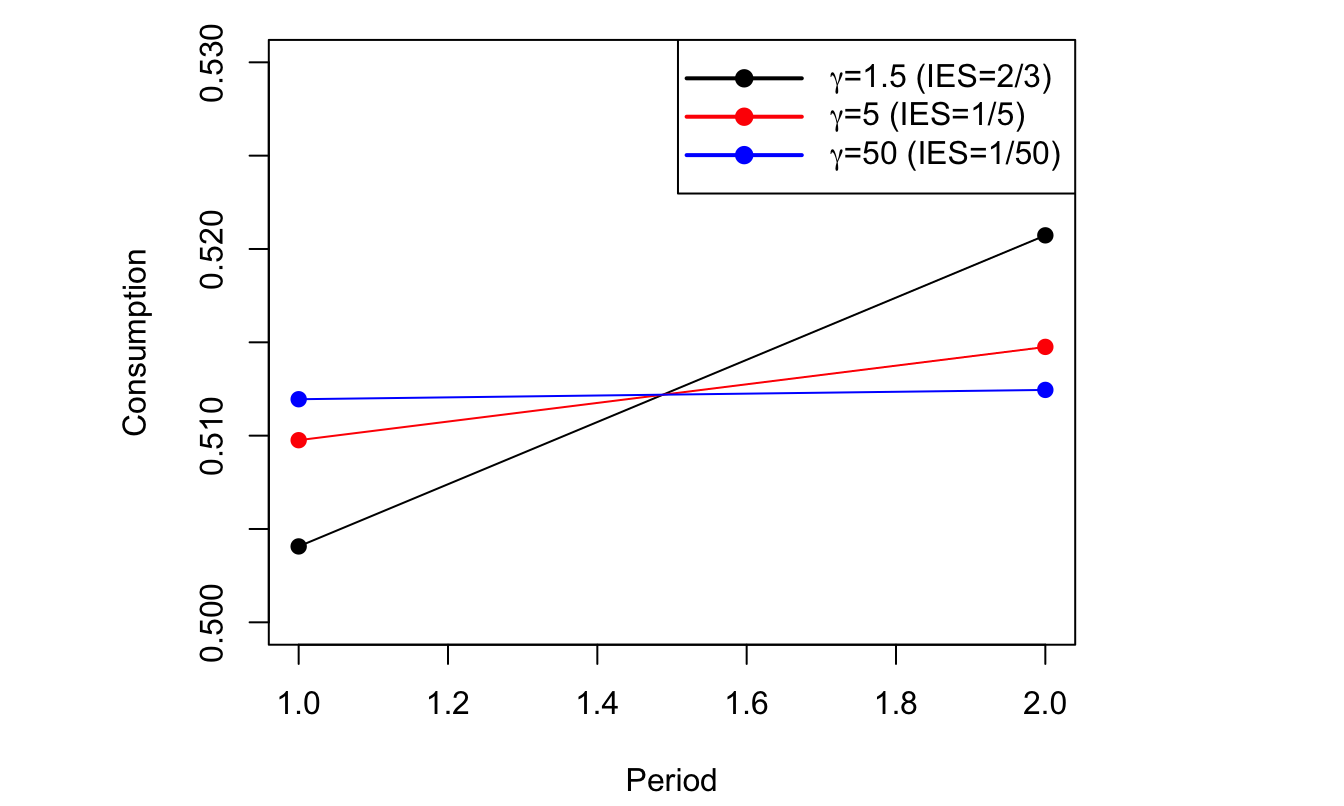
\includegraphics[width=0.95\linewidth]{TSM_files/figure-latex/IESsmooth-1} \caption{Power utility situation. IES and consumption smoothing.}\label{fig:IESsmooth}
\end{figure}

\end{example}

A third problem pertains to the volatility of the SDF

XXX We have
\begin{eqnarray*}
P_{i,t} = \underbrace{\frac{1}{1 + R_{f,t}} \mathbb{E}_t(x_{i,t+1})}_{\mbox{Discount.  expect. payoff}} + \mathbb{V}ar_t(M_{t,t+1}) \underbrace{\frac{\mathbb{C}ov_t(M_{t,t+1},x_{i,t+1})}{\mathbb{V}ar_t(M_{t,t+1})}}_{\mbox{Risk exposure}}
\end{eqnarray*}
or
\begin{equation}
\boxed{\mathbb{E}_t(R_{i,t+1} - R_{f,t}) = - (1 + R_{f,t}) \mathbb{C}ov_t(M_{t,t+1},R_{i,t+1}).}\label{eq:MRCov}
\end{equation}

\citet{Grossman_Shiller_1981} and \citet{Hansen_Jagannathan_1991}: Sharpe ratios give lower bounds to the volatility of SDF:
\[
\frac{\sigma_t(\mathcal{M}_{t,t+1})}{\mathbb{E}_t(\mathcal{M}_{t,t+1})} \ge \underbrace{\frac{\mathbb{E}_t(R_{i,t+1}-R_{f,t})}{\sigma_t(R_{i,t+1})}}_{\mbox{Sharpe ratio of asset $i$.}}
\]
(results from Eq. \eqref{eq:MRCov}, using the fact that \(\mathbb{C}ov(X,Y) \le \sigma(X)\sigma(Y)\))
For postwar U.S. stock market, the Sharpe ratio is about 50\% {[}Table \ref{fig:Campbell1}{]}. Given that \(\mathbb{E}_t(\mathcal{M}_{t,t+1}) \approx 1\), this implies that the volatility of the SDF should be at least 50\%.
For a power utility function {[}Def. \ref{def:RAmeasures}{]}:
\[
\mathcal{M}_{t,t+1}=\delta (C_t/C_{t+1})^\gamma \approx (1 - \gamma \Delta c_{t+1}).
\]
Given the small volatility of \(\Delta c_{t+1}\) {[}column \(\sigma(\Delta c)\) in Table \ref{fig:Campbell1}{]}, \(\gamma\) should be very high for the SDF volatility to be equal to 50\%.

Econometric Test of the C-CAPM: GMM

\citet{Hansen_Singleton_1982} have developed and used the General Method of Moments to test the C-CAPM.
This approach is based on the equation {[}Eq. \eqref{eq:pricingcapm}{]}:
\begin{equation}
1 = \color{red}{\mathbb{E}_t}\left( \delta \left(\frac{C_t}{C_{t+1}}\right)^\gamma (1+R_{i,t+1})\right).\label{eq:momentcondi}
\end{equation}
For this to be verified, we must have, for any variable \(z_t\):
\begin{equation}
\color{red}{\mathbb{E}}\left( \underbrace{\left[\delta \left(\frac{C_t}{C_{t+1}}\right)^\gamma (1+R_{i,t+1}) - 1\right] z_t}_{h_{t+1}}\right) = 0,\label{eq:GMM}
\end{equation}
If this is not the case, one can use \(z_t\) to predict \(\delta \left(\frac{C_t}{C_{t+1}}\right)^\gamma (1+R_{i,t+1})\) and Eq. \eqref{eq:momentcondi} is not valid. Moment condition: \(\mathbb{E}(h_{t+1})=0\).

Empirical counterpart of the moment condition \eqref{eq:GMM}:
\begin{equation}
\frac{1}{T}\sum_{t=1}^{T} \left[\hat\delta \left(\frac{C_t}{C_{t+1}}\right)^{\hat\gamma} (1+R_{i,t+1}) - 1\right] \times\underbrace{z_{j,t}}_{\mbox{instrument}} = 0.
\end{equation}
In order to identify \(\delta\) and \(\gamma\), one need at least two such equations (with some \(z_{1,t}\) and \(z_{2,t}\)).
\citet{Hansen_Singleton_1982} used lagged values of \(R_{i,t+1}\) as instruments. {[}New York Stock Exchange indexes + indexes for different industries{]}

If we have more than 2 equations, we are in a situation of over-identification. One can use over-identifying restrictions to test for the model.

Economically meaningful estimates with \(\gamma\) (\(=-\hat\alpha\) in the table below) close to unity (although with a large standard error) and \(\delta\) (\(=\hat\beta\) in the table below) slightly smaller than unity.
However, when applied to more than one stock index, the over-identifying restrictions are generally rejected. The data reject the simple version of CCAPM.

\begin{figure}

{\centering 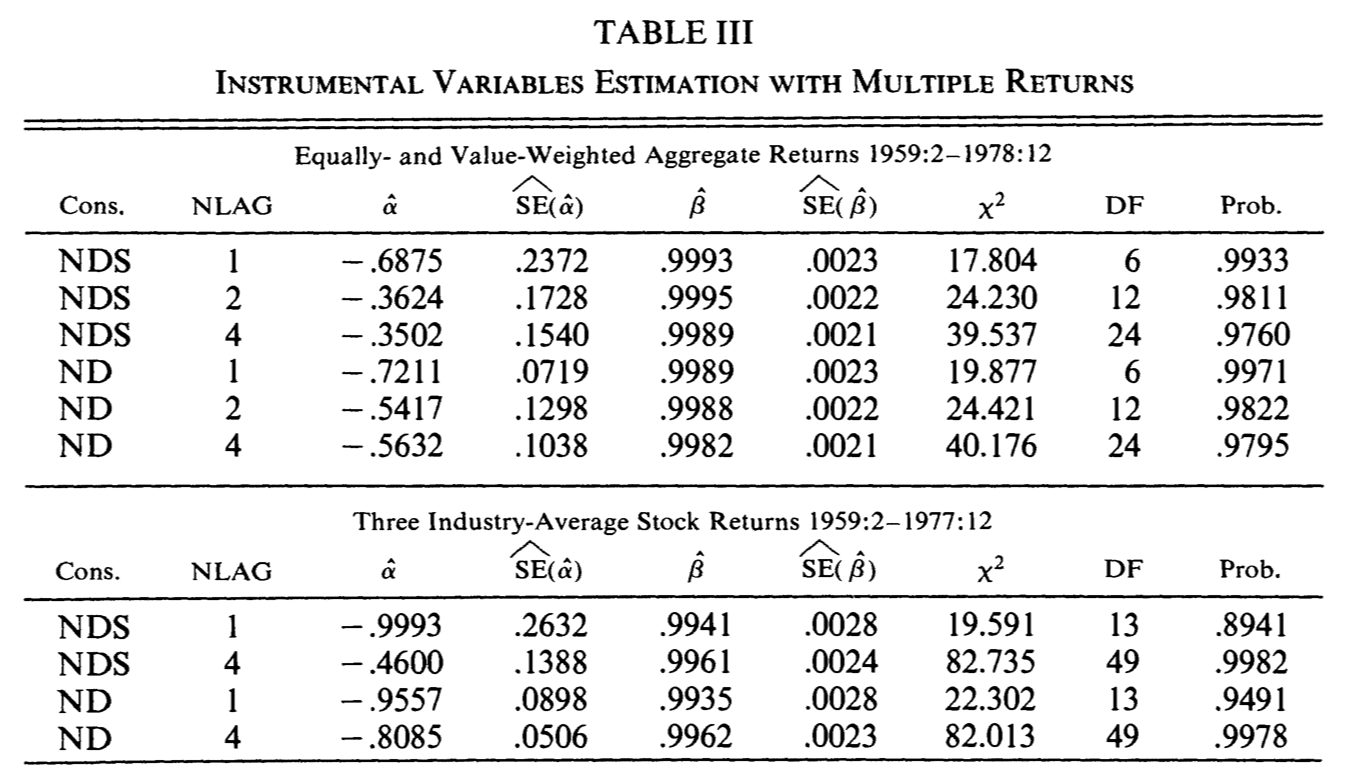
\includegraphics[width=1\linewidth]{figures/tableHansenSingleton82A} 

}

\caption{Source: Hansen and Singleton (1982).}\label{fig:HansenSinfgleton1982}
\end{figure}

\href{https://jrenne.shinyapps.io/APModels}{Web interface}

Long-run horizon

Stocks and consumption are more correlated at low frequencies (see, e.g., this \href{https://jrenne.shinyapps.io/APModels}{web interface}). Hence equity-premium puzzle a little less strong for longer horizons (e.g., \citet{DANIEL_MARSHALL_1997}).
\citet{Jagannathan_Wang_2007}: CAPM not so bad when using fourth-quarter over fourth-quarter non-durable and service consumption {[}see next slide{]}.

Explanation?: A lot of purchases happen at Christmas, with an annual planning horizon (monthly horizon is maybe not relevant).

Time aggregation = Spurious effect {[}Slide @ref(slide:spuriousXS\}{]}? Maybe. But average excess returns line up \(\Rightarrow\) there is something here.

\citet{Parker_Julliard_2005}: study whether the 25 Fama-French portfolios can be priced when considering their exposure to ``long-run'' consumption risk. Formally, they study the condition:
\[
1 = \mathbb{E}_t \left( \beta \left(\frac{C_{t+k}}{C_t}\right)^{- \gamma} (1 + R_{i,t+1})(1 + R_{f,t+1})\times (1 + R_{f,t+k-1}) \right).
\]

C-CAPM: That bad?

\emph{Should we completely discard C-CAPM and the likes?}

\citet{Cochrane_2005}: The failure of the C-CAPM models is quantitative, not qualitative. In particular:

\begin{itemize}
\tightlist
\item
  Signs are consistent: since stock returns are positively correlated to consumption growth, the premiums have to be positive (which they are).
\item
  The decrease in bond term premiums over the last decades is consistent with decrease in the correlation between long-term bond excess returns and consumption {[}e.g.,\href{https://jrenne.shinyapps.io/APModels}{web interface}{]}.
\item
  In terms of signs, the CAPM is also consistent with currency risk premiums {[}see SLIDE FX{]}:
\end{itemize}

\citet{Lustig_Verdelhan_2007} show that high interest rate currencies depreciate on average when domestic consumption growth is low \(\Rightarrow\) the CAPM predicts higher average return for investments in foreign high-interest rate currencies.

\begin{figure}
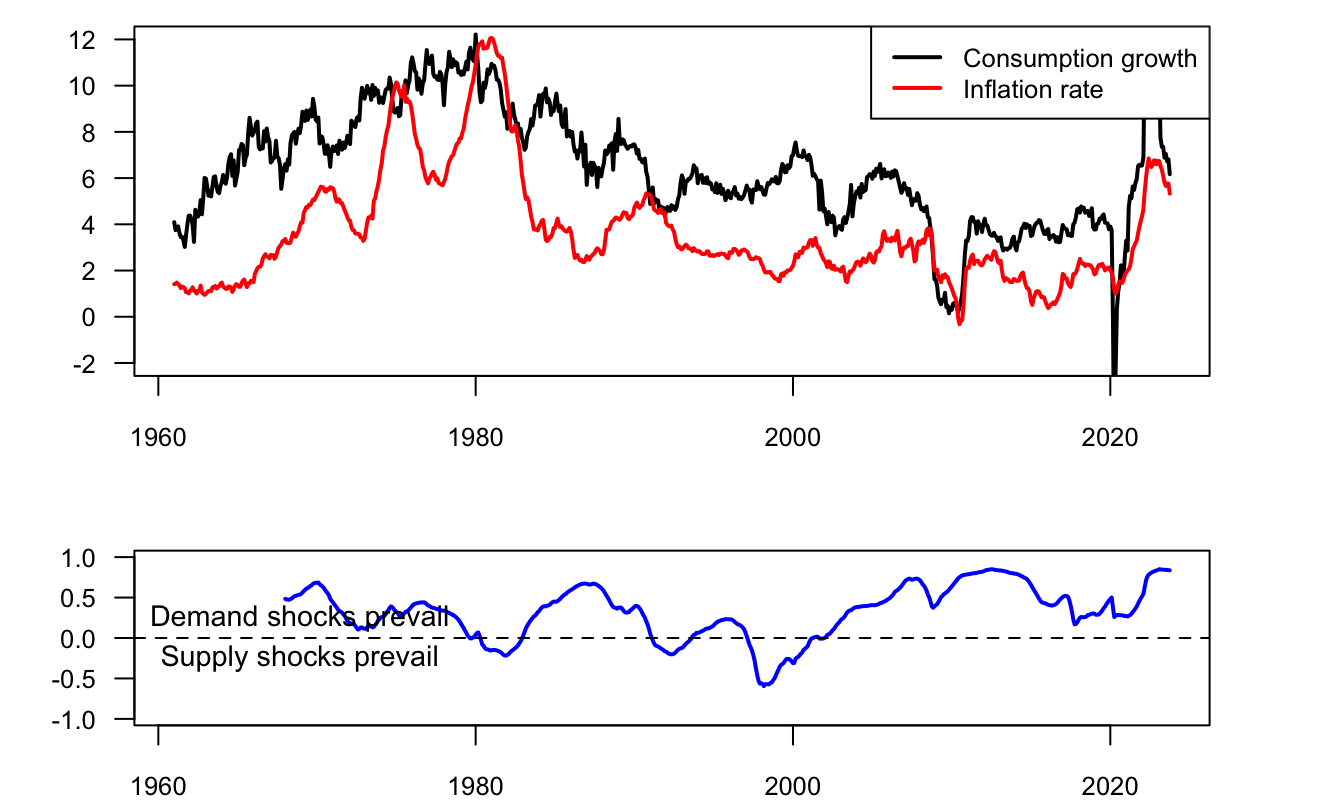
\includegraphics[width=0.95\linewidth]{TSM_files/figure-latex/fredCorrel-1} \caption{Consumption-Inflation correlation. Growth rates are 2-year growth rates. Dynamic correlation is computed using a 7-year rolling window.}\label{fig:fredCorrel}
\end{figure}

\hypertarget{recursive-utilities-and-epstein-zin-preferences}{%
\section{Recursive Utilities and Epstein-Zin Preferences}\label{recursive-utilities-and-epstein-zin-preferences}}

Given the problems of the consumption-based models, one has questioned the utility function (e.g., \citet{Cochrane_2005}). The functional form is not really an issue: in the time-separable framework, linearized and non-linearized models behave relatively similarly. (Utility functions are monotonously increasing with negative second order derivatives.) What about the arguments of the utility function?

\textbf{Idea}: The marginal utility of consumption may not depend only on today's consumption. Pricing implications are very different when the marginal utility of consumption depends past or (expected) future consumption.

\begin{definition}[Expected Utility Time-Separable Preferences]
\protect\hypertarget{def:EUTSpref}{}\label{def:EUTSpref}In the context of \emph{expected utility time-separable preferences}, the intertemporal utility \(U_t\) is defined as:
\[
U_t = \mathbb{E}_t\left(\sum_{i=0}^{\infty} \delta^{i}u(C_{t+i})\right),
\]
or, equivalently, as:
\[
U_t = u(C_t) + \delta \mathbb{E}_t\left(U_{t+1}\right).
\]
\end{definition}

Implications of expected utility time-separable preferences:

\begin{itemize}
\tightlist
\item
  No premium for early resolution of uncertainty.
\item
  As of date \(t\), the promise to know \(C_{t+h}\) at date \(t+1\) has no value.
\item
  No utility effect of potential autocorrelation in \(C_t\).
\item
  Each stream of consumption intervenes independently from the others in the utility computation.
\end{itemize}

What does \emph{non-separability over time} means?

That the marginal utility of today's consumption depends on past consumption. In other words, what you consumed yesterday can have an impact on how you feel about more consumption today.\footnote{As \citet{Cochrane_2005} puts it: ``\emph{Yesterday's pizza lowers the marginal utility for another pizza today.}'')}

A first example is that of \emph{habit formation} \citep{Campbell_Shiller_1999}
\begin{equation}
U_t = \sum_{s=t}^{\infty} \delta^{s-t} u(C_s - X_s) \quad where \quad X_t = \rho X_{t-1} + \lambda C_t.(\#eq:Uhabit_nonstoch)
\end{equation}

The date-\(t\) utility associated with a level of consumption \(C_t\), that is \(u(C_t - X_t)\), is lower is you already had a high level of consumption at date \(t-1\) (high \(X_t\)).
\[
U_t = \sum_{h=0}^{\infty} \delta^{h}u\left(C_{t+h} - \lambda \sum_{j=0}^\infty \rho^j C_{t+h-j}\right).
\]

A fall in consumption hurts after a few years of good times (even if the same level of consumption would have been very pleasant if it arrived after a few bad years).

Without the external habit assumption, the Euler equation (equilibrium relationship between risk-free short-term rate and marginal utilities) is far less tractable:
\begin{eqnarray*}
&& 0 = \Delta U_t / \varepsilon =\\
&& \underbrace{ - u'\left(C_{t} - \lambda \sum_{j=0}^\infty \rho^j C_{t-j}\right) + \lambda  \sum_{h=0}^{\infty} \rho^h \delta^{h}u'\left(C_{t+h} - \lambda \sum_{j=0}^\infty \rho^j C_{t+h-j}\right)}_{\mbox{decrease in utility stemming from lower consumption at date $t$}} +\\
&& \underbrace{\delta(1+R_{f,t}) u'\left(C_{t+1} - \lambda \sum_{j=0}^\infty \rho^j C_{t+1-j}\right) - \lambda (1+R_{f,t}) \sum_{h=1}^{\infty} \rho^h \delta^{h}u'\left(C_{t+h} - \lambda \sum_{j=0}^\infty \rho^j C_{t+h-j}\right)}_{\mbox{increase in utility stemming from higher consumption at date $t+1$}}
\end{eqnarray*}

(Formula derived in the context where we decrease \(C_t\) by \(\varepsilon\) and increase \(C_{t+1}\) by \(\varepsilon(1+R_{f,t})\).)

If one assumes that \(X_t\) is exogenous (external habits) and if \(u(Z)=Z^{1-\gamma}/(1-\gamma)\) (Def. \ref{def:power}) then:
\begin{equation}
\mathcal{M}_{t,t+1} = \delta \left( \frac{C_{t+1}}{C_t} \right)^{-\gamma}\left( \frac{S_{t+1}}{S_t} \right)^{-\gamma},\label{eq:Mhabit}
\end{equation}
where \(S_t = (C_t - X_t)/C_t\).
This extends the standard power utility case by adding an additional state variable (\(X_t\)).
In this model, recessions are periods where consumption is closer to habits (otherwise it is higher).
Specification of the SDF as in Eq. \eqref{eq:Mhabit} can arise in more general contexts (not necessarily habits); \(S_t\) may for instance reflect a business-cycle-related variable.

\begin{example}[Comparisons of situations according to habit preferences]
\protect\hypertarget{exm:habit}{}\label{exm:habit}To illustrate, consider the following context (with no uncertainty):
\[
\delta = 1,\quad \gamma = 3, \quad \rho = 0.5, \quad \lambda = 0.49.
\]
Let's define two sequences of interest rates (A and B):
\begin{eqnarray*}
R^{(A)}_1 &=&R^{(A)}_2 =\dots=R^{(A)}_5 =  7\% \\
R^{(A)}_6 &=&R^{(A)}_7 =R^{(A)}_8 =  -20\%
\end{eqnarray*}
and
\[
R^{(B)}_1 =R^{(B)}_2 =\dots=R^{(B)}_{10} =  2.5\%.
\]
For each sequence, we compute the resulting sequence of consumption, with \(C_1=1\).
Results on next slide.

\begin{figure}
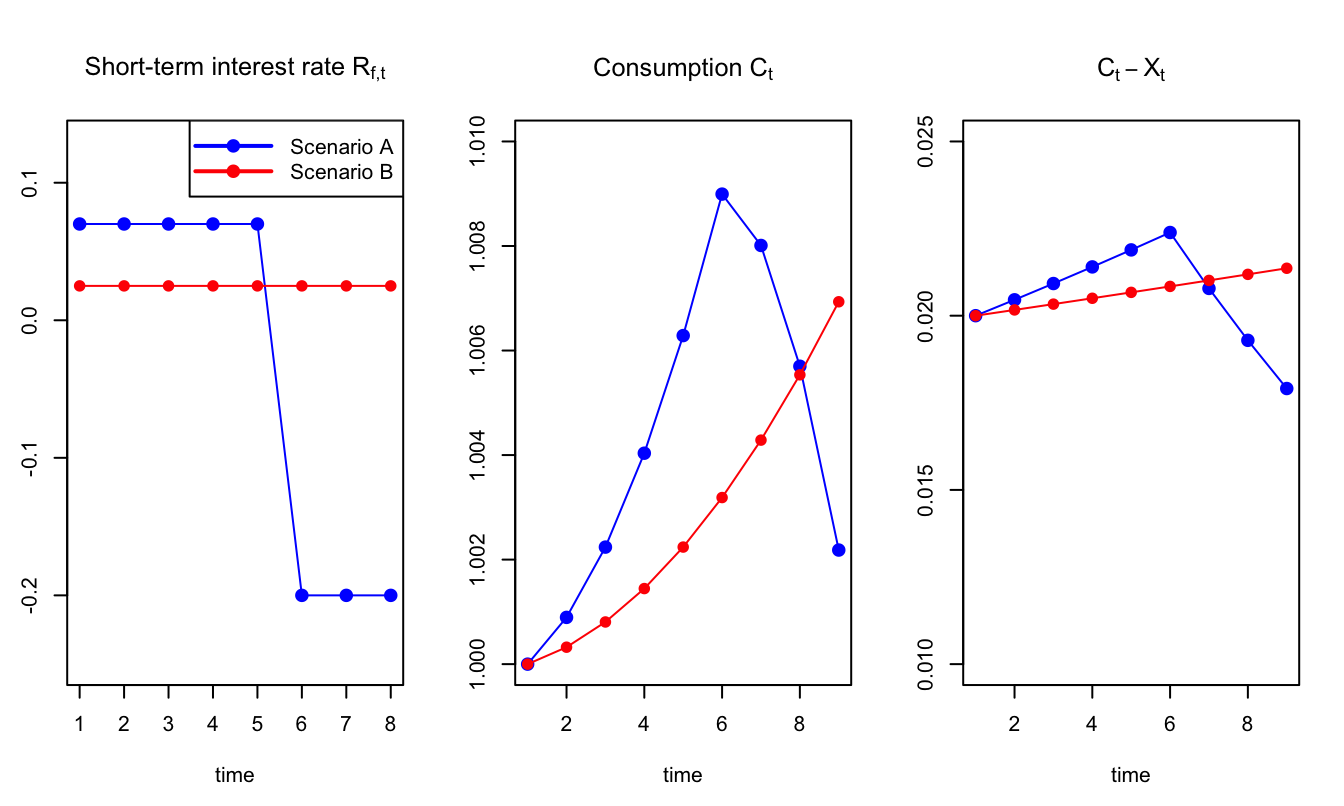
\includegraphics[width=0.95\linewidth]{TSM_files/figure-latex/Habits1-1} \caption{Comparison of scenarios A and B using habit-based preferences.}\label{fig:Habits1}
\end{figure}

The utility associated to Scenario A (\(-10779\)) is lower than that associated to Scenario B (\(-10542\)).
Without the \(X_t\) term, the utility of Scenario A would be higher than that of Scenario B.
\end{example}

\hypertarget{limitations-of-the-habit-models-for-long-horizons}{%
\subsection{Limitations of the Habit Models for Long-Horizons}\label{limitations-of-the-habit-models-for-long-horizons}}

The models based on Eq. \eqref{eq:Mhabit} generally works well in the short-run but not in the long-run. Let us consider the horizon-\(h\) SDF:
\[
\mathcal{M}_{t,t+h} = \delta \left( \frac{C_{t+h}}{C_t} \right)^{-\gamma}\left( \frac{S_{t+h}}{S_t} \right)^{-\gamma},
\]
In order to generate a high maximum Sharpe ratio for long horizons, we need a high conditional volatility of \(\mathcal{M}_{t,t+h}\).
If \(c_t\) follows a random walk, the volatility of \(\left( \frac{C_{t+h}}{C_t} \right)^{-\gamma}\) is approximately linear in \(h\).
By contrast, if \(S_t^{-\gamma}\) is stationary, then the conditional volatility of \(\left( \frac{S_{t+h}}{S_t} \right)^{-\gamma}\) does not increase indefinitely with \(h\) (though this term may substantially contribute to the short-run SDF volatility).
{[}\(\Rightarrow\){]} For long-run horizons, these models do not solve the problems pertaining to the standard power utility time-separable model.

\citet{Epstein_Zin_1989} have proposed a framework where

\begin{itemize}
\tightlist
\item
  there is a premium for early resolution and
\item
  the time composition of risk matters.
\end{itemize}

\begin{definition}[Epstein and Zin (1989) Preferences]
\protect\hypertarget{def:EZ}{}\label{def:EZ}Epstein-Zin preferences are defined recursively over current (known) consumption and a certainty equivalent
\(R_t(U_{t+1})\) {[}Def. \ref{def:CE}{]} of future utility:
\[
U_{t} = F(C_t,R_t(U_{t+1})),
\]
where \(R_t(U_{t+1})\), the certainty equivalent of \(U_{t+1}\), is:
\[
R_t(U_{t+1}) = G^{-1}[\mathbb{E}_t(G(U_{t+1}))],
\]
where \(F\) and \(G\) are increasing and concave functions, and where \(F\) is homogenous of degree one.
\end{definition}

\begin{quote}
We have \(R_t(U_{t+1})=\mathbb{E}_t(U_{t+1})\) if \(G\) is linear.
\end{quote}

\begin{quote}
We have \(R_t(U_{t+1})=U_{t+1}\) if \(U_{t+1}\) is not random.
\end{quote}

Standard functions \(F\) and \(G\) (with \(\rho\) and \(\gamma\) \(>0\)):
\[
F(c,v) = \left((1-\delta)c^{1-\rho} + \delta v^{1-\rho}\right)^{\frac{1}{1-\rho}}, \quad G(x)=\frac{x^{1-\gamma}}{1-\gamma},
\]
In this case:
\begin{equation}
\boxed{ U_t = \left((1-\delta)C_t^{1-\rho}+\delta \left[\underbrace{ \mathbb{E}_t\left(U_{t+1}^{1-\gamma}\right)^{\frac{1}{1-\gamma}} }_{\mbox{certainty equivalent}}\right] ^{1-\rho}\right)^{\frac{1}{1-\rho}}.}\label{eq:EZpreferences}
\end{equation}
or
\[
U_t = \left((1-\delta)C_t^{1-\rho} + \delta R_t(U_{t+1})^{1-\rho}\right)^{\frac{1}{1-\rho}}.
\]
where \(R_t(U_{t+1})=\mathbb{E}_t(U_{t+1}^{1-\gamma})^{\frac{1}{1-\gamma}}\).

\begin{quote}
\textbf{Case \(\gamma = \rho\)}. If \(\gamma = \rho\), \(U_t^{1-\rho}=(1-\delta)C_t^{1-\rho} + \delta \mathbb{E}_t(U_{t+1}^{1-\rho})\).
Divide by \(1-\rho\) and replace \(U_t^{1-\rho}/(1-\rho)\) by \(W_t\)
{[}\(\Rightarrow\){]} Back to the expected utility case {[}see Def. \ref{def:EUTSpref}{]}.
\end{quote}

\hypertarget{epstein-zin-preferences-and-risk-aversion}{%
\subsection{Epstein-Zin Preferences and Risk Aversion}\label{epstein-zin-preferences-and-risk-aversion}}

\(\gamma\) is the \emph{relative risk aversion} {[}Def. \ref{def:RAmeasures}{]} parameter.
Consider the following context:

\begin{itemize}
\tightlist
\item
  At date 0, the agent consumes \(C_0\).
\item
  At date 1, he consumes \(C_h\) (high) with probability \(1/2\) and \(C_l\) (low) with probability \(1/2\).
\item
  In the subsequent periods, he consumes 0.
\end{itemize}

We have \(U_2 = 0\) and
\[
U_1 = U_h = (1-\delta)^{\frac{1}{1-\rho}}C_h \mbox{ with probability 1/2}
\]
and
\[
U_1 = U_l = (1-\delta)^{\frac{1}{1-\rho}}C_l \mbox{ with probability 1/2}.
\]
Therefore
\[
U_0 =  \left((1-\delta)C_0^{1-\rho} + \delta \left(\frac{1}{2}U_h^{1-\gamma}+\frac{1}{2}U_l^{1-\gamma}\right)^{\frac{1-\rho}{1-\gamma}}\right)^{\frac{1}{1-\rho}}.
\]

What is the certainty equivalent \(C_1\) to the period-1 gamble? \(C_1\) solves:
\[
U_0 = \left((1-\delta)C_0^{1-\rho} + \delta (1-\delta) C_1^{1-\rho}\right)^{\frac{1}{1-\rho}},
\]
that is:
\[
C_1 = \left(\frac{1}{2}C_h^{1-\gamma}+\frac{1}{2}C_l^{1-\gamma}\right)^{\frac{1}{1-\gamma}}.
\]
This certainty equivalent is the same as the one that one would get if the utility function was the standard (time-separable) power utility function (with RRA \(= \gamma\)).
{[}\(\Rightarrow\){]} \(\gamma\) measures agents' relative risk aversion.

Consider the case with two periods (\(0\) and \(1\)) and where \(C_0=0\). We have (up to a multiplicative factor):
\[
U_0 = \left\{\mathbb{E}_0(C_{1}^{1-\gamma})\right\}^{\frac{1}{1-\gamma}}.
\]
At date 1, the agent will consume \(C_1 = \kappa(1+X)\), where \(X \sim \mathcal{N}(0,\sigma^2)\) and \(\sigma^2<<1\). We have
\begin{eqnarray*}
U_0 &=& \left\{\mathbb{E}_0(C_{1}^{1-\gamma})\right\}^{\frac{1}{1-\gamma}}\\
&=& \left\{\mathbb{E}_0(\exp([1-\gamma]\ln(C_1)))\right\}^{\frac{1}{1-\gamma}}\\
&\approx& \left\{\mathbb{E}_0(\exp([1-\gamma][\ln(\kappa) + X - X^2/2 + o(X^2)]))\right\}^{\frac{1}{1-\gamma}}\\
&\approx& \kappa \left\{\mathbb{E}_0(\exp([1-\gamma][X-X^2/2 + o(X^2)]))\right\}^{\frac{1}{1-\gamma}}\\
&\approx& \kappa (1-\gamma\sigma^2/2).
\end{eqnarray*}
{[}\(\Rightarrow\){]} \(\gamma\): measure of risk aversion.

\hypertarget{epstein-zin-preferences-and-ies}{%
\subsection{Epstein-Zin Preferences and IES}\label{epstein-zin-preferences-and-ies}}

In the deterministic context,
\[
U_t = \left((1-\delta)C_t^{1-\rho} + \delta U_{t+1}^{1-\rho}\right)^{\frac{1}{1-\rho}}.
\]
And, setting \(W_t = U_t^{1-\rho}/(1-\rho)\), we have:
\[
W_t = (1-\delta)\frac{C_t^{1-\rho}}{1-\rho} + \delta W_{t+1} = (1-\delta)\frac{C_t^{1-\rho}}{1-\rho} + \delta(1-\delta)\frac{C_{t+1}^{1-\rho}}{1-\rho} + \delta^2 W_{t+2}.
\]
Maximizing \(U_t\) is equivalent to maximizing \(W_t\). In that context, one can show that:
\[
\frac{1}{1+ R_{f,t}}=\delta \left(\frac{C_{t+1}}{C_t}\right)^{-\rho}.
\]
Hence, as for the standard power utility case, one obtains that \(IES = 1/\rho =: \psi\) {[}IES Def. \ref{def:IES}{]}.

\begin{quote}
Crucially, with Epstein-Zin preferences, the risk aversion (\(\gamma\)) and the IES (\(\psi=1/\rho\)) are controlled by two independent parameters.
\end{quote}

\hypertarget{epstein-zin-preferences-and-the-time-composition-of-risk}{%
\subsection{Epstein-Zin Preferences and the Time Composition of Risk}\label{epstein-zin-preferences-and-the-time-composition-of-risk}}

Let's compare two lotteries:

\begin{itemize}
\tightlist
\item
  \textbf{Lottery A}: There is single draw at \(t=1\). It pays starting at t = 1 either \(C_h\) at all future dates (probability of 1/2), or \(C_l\) at all future dates (probability of 1/2).
\item
  \textbf{Lottery B}: In each period \(t = 1, 2, \dots\), this lottery pays \(C_h\) with probability 1/2 or \(C_l\) with probability 1/2, the outcomes (\(t = 1, 2, \dots\)) are i.i.d.
\end{itemize}

We also assume that \(C_0=0\).

Intuitively, plan A looks more ``risky'' than plan B.
Plan A: all eggs in one basket; Plan B: more diversified.
If all payoffs were realized at the same time, risk aversion would imply a preference for plan B (even in the standard time-separable expected utility model).
However, if the payoffs arrive at different dates, the standard time-separable expected utility model implies indifference between A and B.

With time-separable utility functions, agents would be indifferent between playing the two lotteries. The reason is that the time-separable model evaluates risks at different dates in isolation \citep{Piazzesi_Schneider_2007}. From the perspective of time zero, random consumption at any given date---viewed in isolation---does have the same risk (measured, for example, by the variance.) For Epstein-Zin preferences (and other recursive preference schemes), the \emph{time-composition of risk} matters.

Let's first consider Lottery A. At date \(t=1\), there will be no uncertainty any more. It is easily seen that, if one draws \(C_i\) (\(i \in \{l,h\}\)) at date 1, then \(U_1^A = C_i\). Hence
\begin{equation}
U_0^A =  \left(\delta \left(\frac{1}{2}C_h^{1-\gamma}+\frac{1}{2}C_l^{1-\gamma}\right)^{\frac{1-\rho}{1-\gamma}}\right)^{\frac{1}{1-\rho}}= \delta^{\frac{1}{1-\rho}} \left(\frac{1}{2}C_h^{1-\gamma}+\frac{1}{2}C_l^{1-\gamma}\right)^{\frac{1}{1-\gamma}}.\label{eq:U0A}
\end{equation}
For lottery B, at each period (\(t\ge1\)), there are two possible utility outcomes: \(V_h\) or \(V_l\).
Specifically, if, at date 1, we get \(C_i\) (\(i \in \{l,h\}\)), the utility is:
\begin{equation}
U_1^B = V_i = \left((1-\delta)C_i^{1-\rho} + \delta \left(\frac{1}{2}V_h^{1-\gamma}+\frac{1}{2}V_l^{1-\gamma}\right)^{\frac{1-\rho}{1-\gamma}}\right)^{\frac{1}{1-\rho}}\label{eq:ABCD}
\end{equation}
and, for date 0:
\[
U_0^B =  \left(\delta \left(\frac{1}{2}V_h^{1-\gamma}+\frac{1}{2}V_l^{1-\gamma}\right)^{\frac{1-\rho}{1-\gamma}}\right)^{\frac{1}{1-\rho}}= \delta^{\frac{1}{1-\rho}}\left(\frac{1}{2}V_h^{1-\gamma}+\frac{1}{2}V_l^{1-\gamma}\right)^{\frac{1}{1-\gamma}}.
\]

Let's compare \(U_0^A\) and \(U_0^B\), i.e.,
\[
\left(\frac{1}{2}C_h^{1-\gamma}+\frac{1}{2}C_l^{1-\gamma}\right)^{\frac{1}{1-\gamma}}
\overset{?}{\ge \le}
\left(\frac{1}{2}V_h^{1-\gamma}+\frac{1}{2}V_l^{1-\gamma}\right)^{\frac{1}{1-\gamma}}.
\]
Consider the case \(\gamma > 1\). We have then:
\begin{eqnarray*}
U_0^A \le U_0^B &\Leftrightarrow& \left(\frac{1}{2}C_h^{1-\gamma}+\frac{1}{2}C_l^{1-\gamma}\right)^{\frac{1}{1-\gamma}} \le \left(\frac{1}{2}V_h^{1-\gamma}+\frac{1}{2}V_l^{1-\gamma}\right)^{\frac{1}{1-\gamma}}\\
&\Leftrightarrow& \frac{1}{2}C_h^{1-\gamma}+\frac{1}{2}C_l^{1-\gamma} \ge \frac{1}{2}V_h^{1-\gamma}+\frac{1}{2}V_l^{1-\gamma},
\end{eqnarray*}
which is verified because \(C_l \le V_l \le V_h \le C_h\) and because, when \(\gamma > 1\), then \(x\rightarrow x^{1-\gamma}\) is convex.

\hypertarget{epstein-zin-preferences-and-early-resolution-uncertainty}{%
\subsection{Epstein-Zin Preferences and Early Resolution Uncertainty}\label{epstein-zin-preferences-and-early-resolution-uncertainty}}

Two new lotteries: C and D; 3 periods are involved: 0, 1 and 2.
The consumption of dates 1 and 2 are determined by independent tosses of a fair coin: either \(C_l\) or \(C_h\).
The difference between Lotteries C and D pertains to the date on which the information about the tosses is revealed: in Lottery C, the outcomes of the two tosses are revealed at date 1. in Lottery D, the \(2\)nd toss is not revealed before date \(2\).
In both cases, we have \(U_2 = (1-\delta)^{\frac{1}{1-\rho}}C_{2}\).
At date 1, we have:
\begin{eqnarray*}
U_1^C &=& \left((1-\delta)C_1^{1-\rho} + \delta U_2^{1-\rho}\right)^{\frac{1}{1-\rho}}\\
U_1^D &=& \left((1-\delta)C_1^{1-\rho} + \delta \mathbb{E}(U_2^{1-\gamma})^{\frac{1-\rho}{1-\gamma}}\right)^{\frac{1}{1-\rho}}.
\end{eqnarray*}
And, therefore:
\begin{eqnarray*}
U_0^C &=& \delta^{\frac{1}{1-\rho}} \mathbb{E}({U_1^C}^{1-\gamma})^{\frac{1}{1-\gamma}}\\
U_0^D &=& \delta^{\frac{1}{1-\rho}} \mathbb{E}({U_1^D}^{1-\gamma})^{\frac{1}{1-\gamma}}.
\end{eqnarray*}

Lottery C: \emph{early resolution of uncertainty} (compared to D).
The difference between \(U_0^C\) and \(U_0^D\) measures the preference for early resolution of uncertainty.
One can show that agents prefer early resolution of uncertainty iff \(RRA = \gamma > 1/IES = \rho\) (e.g., \citet{Epstein_Fahri_Strzalecki_2014} or \citet{Duffie_Epstein_1992}).
Simulations: \(C_l = 0.8\), \(C_h = 1.2\), \(\delta = 0.5\).

\begin{figure}
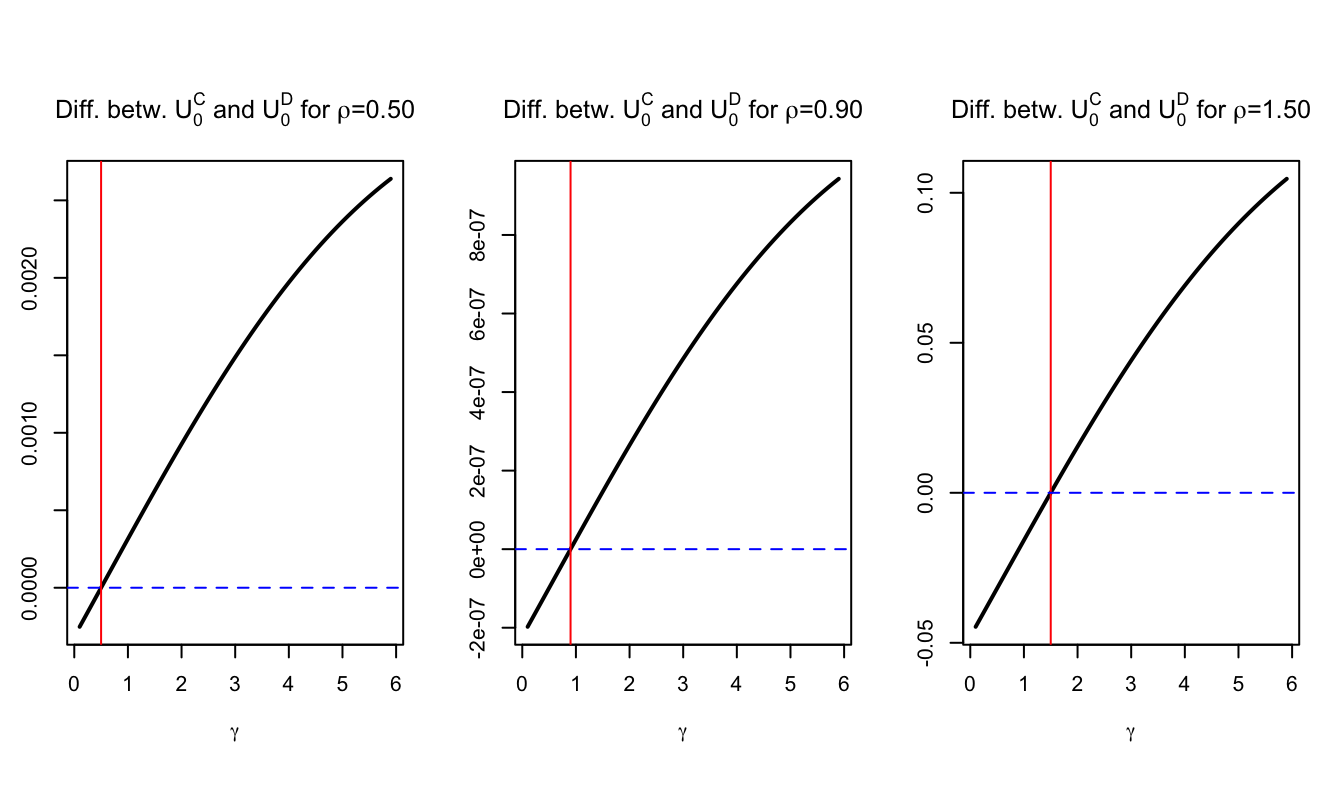
\includegraphics[width=0.95\linewidth]{TSM_files/figure-latex/EZresolution-1} \caption{Comparison of scenarios C and D illustrating the preference for early resolution of uncertainty.}\label{fig:EZresolution}
\end{figure}

\hypertarget{the-sdf-with-epstein-zin-preferences}{%
\subsection{The SDF with Epstein-Zin preferences}\label{the-sdf-with-epstein-zin-preferences}}

Consider an asset that provides the payoff \(x_{t+1}\) at date \(t+1\).
The equilibrium price \(\pi_t(x_{t+1})\) of this asset is such that agents are indifferent between buying or not an additional unit \(\varepsilon\) of this asset.
That is, \(U_t = F(C_t,R_t(U_{t+1}))\) is also equal to:
\begin{eqnarray}
&&  F(C_t,R_t(\color{blue}{U_{t+1}})) \nonumber \\
&=&F(C_t-\varepsilon \pi_t(x_{t+1}),R_t(\color{blue}{F(C_{t+1}+\varepsilon x_{t+1},R_{t+1}(U_{t+2}))})).\label{eq:SDFV}
\end{eqnarray}
This implies:
\[
\pi_t(x_{t+1}) = \mathbb{E}_t \left( x_{t+1} \mathcal{M}_{t,t+1} \right),
\]
where \(\mathcal{M}_{t,t+1}\) is given by:
\begin{equation}
\mathcal{M}_{t,t+1}= \delta \left(\frac{C_{t+1}}{C_t}\right)^{-\rho}  \left(\frac{U_{t+1}}{R_{t}(U_{t+1})}\right)^{\rho-\gamma}.\label{eq:SSS}
\end{equation}
:::\{.proof\}
See Appendix \ref{SDFEZ}.
:::

\(\mathcal{M}_{t,t+1}\) is the SDF, or pricing kernel {[}Def. \ref{def:sdf}{]}.

Recall that, for all asset \(i\) (whose return is \(R_{i,t}\)), we have (Eq. \eqref{eq:MRCov}):
\[
\mathbb{E}_t(R_{i,t+1} - R_{f,t}) = - (1 + R_{f,t}) \mathbb{C}ov_t(\mathcal{M}_{t,t+1},R_{i,t+1}).
\]
Hence, with Eq. \eqref{eq:SSS}, expected returns depend not only on covariances between returns and consumption growth (as in the C-CAPM) but also on covariances between returns and the next period utility index, which captures news about the investor's future prospects.
To make the formula operational, one has to find a proxy for the utility. One can show that this utility is proportional to the value of the ``wealth portfolio''.
Before looking into it, let's look at the implication of Eq. \eqref{eq:SSS} in the simplified context where \(\rho = 1\).

\hypertarget{pricing-information-on-future-consumption-path}{%
\subsection{Pricing Information on Future Consumption Path}\label{pricing-information-on-future-consumption-path}}

Consider the case where \(\rho = 1\) and log-normal conditionally homoskedastic consumption (see Appendix XXX of \citet{Cochrane_2005}).

Using \(v_t = \log(U_t)\), we have:
\[
v_t = (1 - \delta) c_t + \delta \frac{1}{1 - \gamma} \log \mathbb{E}_t \left(\exp((1-\gamma)v_{t+1})\right).
\]
If \(c_t\) is log-normal, one can show that \(v_t\) is log-normal as well. Hence:
\begin{eqnarray}
v_t &=& (1 - \delta) c_t + \delta \mathbb{E}_t(v_{t+1}) + \frac{1}{2}\delta (1-\gamma) \sigma^2(v_{t+1})\nonumber \\
&=& (1 - \delta) \left( \sum_{j=0}^{\infty}  \delta^j \mathbb{E}_t (c_{t+j}) \right) + \frac{1}{2}\delta \frac{1-\gamma}{1-\delta} \sigma^2(v_{t+1}) (\#eq:v_rho1).
\end{eqnarray}

Besides, Eq. \eqref{eq:SSS} gives:
\begin{eqnarray*}
m_{t,t+1} &=& \log(\delta) - \rho \Delta c_{t+1} + (\rho - \gamma) \left(v_{t+1} - \frac{1}{1 - \gamma} \log \mathbb{E}_t \left(\exp((1-\gamma)v_{t+1})\right)\right)\\
&=& \log(\delta) - \rho \Delta c_{t+1} + (\rho - \gamma) \left(v_{t+1} - \mathbb{E}_t(v_{t+1}) - \frac{1}{2} \frac{1-\gamma}{1-\delta} \sigma^2(v_{t+1})\right).
\end{eqnarray*}
Therefore (\(\mathbb{E}_{t+1} - \mathbb{E}_t\) = ``expectation updating'' operator):
\[
(\mathbb{E}_{t+1} - \mathbb{E}_t) m_{t,t+1} = - \rho(\mathbb{E}_{t+1} - \mathbb{E}_t) c_{t+1} + (\rho - \gamma) (\mathbb{E}_{t+1} - \mathbb{E}_t) v_{t+1},
\]
which gives, when \(\rho = 1\) (using Eq. @ref(eq:v\_rho1)):
\begin{eqnarray}
(\mathbb{E}_{t+1} - \mathbb{E}_t) m_{t,t+1} &=& - (\mathbb{E}_{t+1} - \mathbb{E}_t) c_{t+1} +  \\
&& (1 - \gamma)(1 - \delta) (\mathbb{E}_{t+1} - \mathbb{E}_t) \left(  \sum_{j=1}^{\infty}  \delta^j c_{t+j}  \right).\nonumber
\end{eqnarray}

The previous equation can be rewritten as:
\begin{eqnarray}
&& (\mathbb{E}_{t+1} - \mathbb{E}_t) m_{t,t+1} \nonumber \\
&=& - \gamma(\mathbb{E}_{t+1} - \mathbb{E}_t)\Delta c_{t+1} +  \label{eq:sdfAbc}\\
&&  (1 - \gamma) \times \underbrace{ (\mathbb{E}_{t+1} - \mathbb{E}_t) \left(  \sum_{j=1}^{\infty}  \delta^j \Delta c_{t+1+j}  \right).}_{\mbox{innovation in long-run consumption growth}}\nonumber
\end{eqnarray}
News about future consumption growth affect current SDF (marginal rate of substitution).
{[}\(\Rightarrow\){]} Shocks that correlate with updates of future consumption growth are ``priced''.

Assets are priced by covariance with current \emph{and} future consumption growth.

\begin{quote}
If consumption is a random walk, then EZ preferences are observationally equivalent to power utility \citep{Kocherlakota_1990}.
\end{quote}

Consider the case where \(C_0 = C_1 = 1\).
At date \(t=1\), one get information about future consumption levels:

\begin{itemize}
\tightlist
\item
  {[}Case I{]} With probability 0.50, one will have \(C_t=\exp(\omega)\) for \(t\ge2\)
\item
  {[}Case II{]} With probability 0.50, one will have \(C_t=\exp(-\omega)\) for \(t\ge2\)
\end{itemize}

where \(\omega \ge 0\).
Eq. \eqref{eq:sdfAbc} implies that:
\[
m_{0,1} = \mathbb{E}_0(m_{0,1}) + (1 - \gamma)\delta \Delta c_{2}.
\]
(using that \(\mathbb{E}_0(\Delta c_{2})=0\) and that \(\mathbb{E}_1(\Delta c_{2})=\Delta c_{2}\).)
Assume that \(\mathbb{E}_0(m_{0,1})\) is such that \(\mathbb{E}_0(\mathcal{M}_{0,1})=\mathbb{E}_0(\exp(m_{0,1}))=1\) (i.e.~the risk-free rate is 0).
We consider the price of an asset that provides 1 at date 1 under Case II and 0 under Case I.
The price of this asset is:
\[
\mathbb{E}_t(\mathcal{M}_{t,t+1}\mathbb{I}_{\{Case II\}}) = \frac{1}{2} \times e^{\mathbb{E}_0(m_{0,1}) - (1 - \gamma)\delta \omega} \times 1.
\]

The plots below show the price of this asset for different values of \(\gamma\) and \(\omega\) (\(\delta=0.9\)).
With expected utility time-separable preferences {[}Def. \ref{def:EUTSpref}{]} the price of such an asset would be 0.50 (blue dashed line).

\begin{figure}
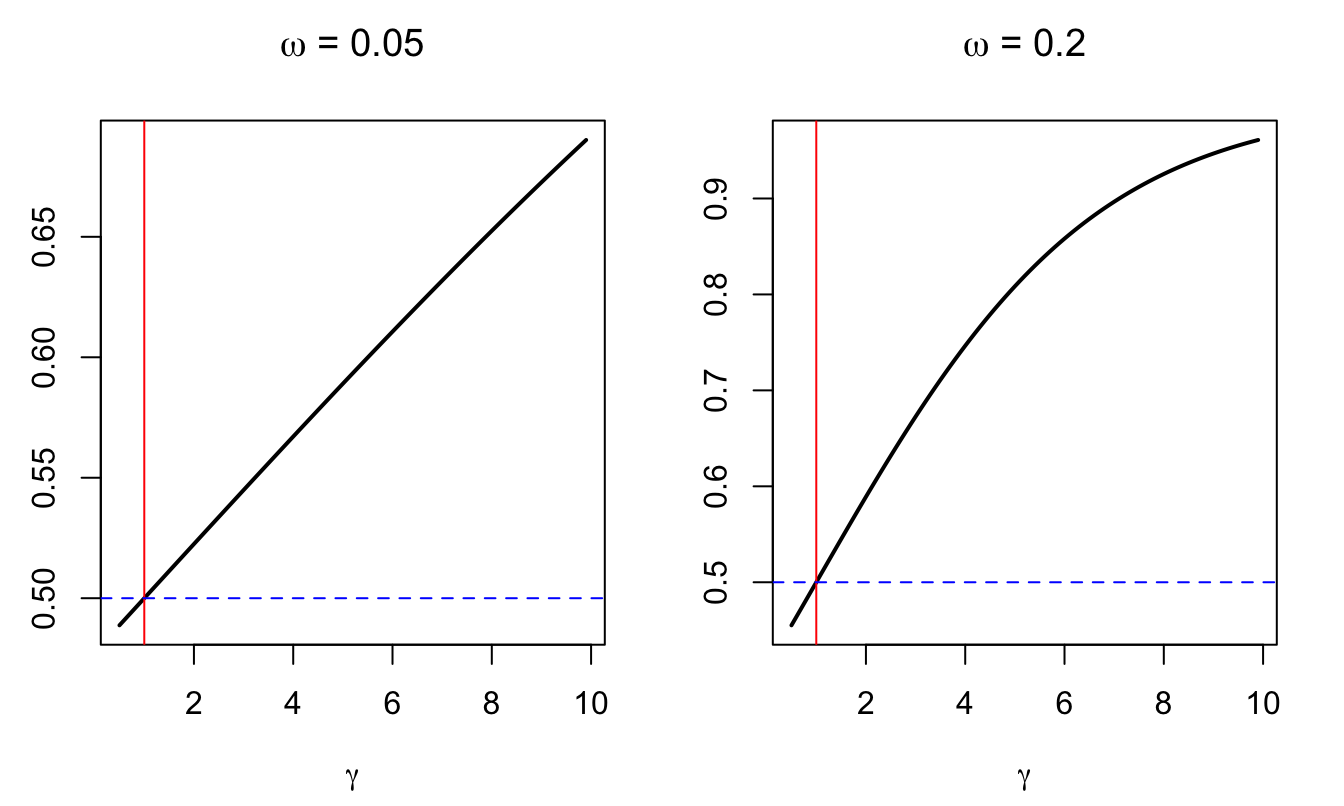
\includegraphics[width=0.95\linewidth]{TSM_files/figure-latex/EZresolution2-1} \caption{Price of an asset that pays 1 under Case II.}\label{fig:EZresolution2}
\end{figure}

\hypertarget{rewriting-the-sdf-with-epstein-zin-preferences}{%
\subsection{Rewriting the SDF with Epstein-Zin Preferences}\label{rewriting-the-sdf-with-epstein-zin-preferences}}

Because \(F\) is homogenous of degree one in its arguments (\(C_t\) and \(R_t(U_{t+1})\)), the Euler's theorem yields \citep{HANSEN20073967}:
\begin{equation}
U_t = C_t \frac{\partial U_t}{\partial C_t} +  R_t(U_{t+1}) \frac{\partial U_t}{\partial R_t(U_{t+1})}.\label{eq:XXYXX}
\end{equation}
Taking the current consumption as numeraire, the wealth \(W_t\) is defined by:
\begin{equation}
W_t =   U_t \frac{\partial U_t}{\partial C_t}.\label{eq:WWWWW}
\end{equation}
Interpretation of \(W_t\)?

\(F\) homogeneous of order 1 \(\Rightarrow\) if all future consumption streams are multiplied by \(1+\epsilon\), then the utility becomes \((1+\epsilon)U_t\).
Consider the asset that provides \(\epsilon C_{t+h}\) at all future periods (if one purchases \(\epsilon\) units of it).
Expressed in consumption units, the equilibrium unit price \(W_t\) of this asset must satisfy \(-\epsilon U_t + \epsilon W_t (\partial U_t / \partial C_t)=0\) \(\Rightarrow\) Eq. \eqref{eq:WWWWW}.

{[}\(\Rightarrow\){]} If you want to trade all your future consumption against current consumption, you will consume \(W_t\) at date \(t\).

\(W_t\) can be seen as a consumption-priced virtual asset that delivers aggregate consumption as its dividends on each time period. This asset is called wealth portfolio.
After computation {[}using Eq. \eqref{eq:XXYXX}{]}:
\begin{equation}
W_t = \frac{U_t^{1-\rho}C_t^\rho}{1 - \delta}.\label{eq:WWW}
\end{equation}
Let's denote by \(R_{a,t+1}\) the return on the wealth portfolio. We have:
\begin{equation}
1+R_{a,t+1} := \frac{W_{t+1}}{W_t - C_t} = \frac{P_{a,t+1}+C_{t+1}}{P_{a,t}},\label{eq:Ra}
\end{equation}
where \(P_{a,t} := W_t - C_t\).

Using Eq. \eqref{eq:WWW}, it can be shown that:
\[
1+R_{a,t+1} = \left[ \delta \left( \frac{C_{t+1}}{C_t} \right)^{-\rho} \left( \frac{R_t(U_{t+1})}{U_{t+1}} \right)^{1-\rho} \right]^{-1},
\]
which is equivalent to:
\[
\frac{U_{t+1}}{R_t(U_{t+1})} = \left[ \delta (1+ R_{a,t+1}) \left( \frac{C_{t+1}}{C_t} \right)^{-\rho}  \right]^{\frac{1}{1-\rho}}.
\]
Substituting in Eq. \eqref{eq:SSS} gives:
\begin{equation}
\mathcal{M}_{t,t+1} =  \delta^{\theta} (1+R_{a,t+1})^{\theta - 1} \left( \frac{C_{t+1}}{C_t} \right)^{- \frac{\theta}{\psi}}
\end{equation}
where
\[
\theta = \frac{1-\gamma}{1-\rho} \quad and \quad \psi = \frac{1}{\rho}.
\]
Therefore (using \(\exp(r_{a,t+1})=1+R_{a,t+1}\)):
\begin{equation}
\boxed{\log(\mathcal{M}_{t,t+1}) = \theta \log \delta - \frac{\theta}{\psi} \Delta \log(C_{t+1}) - (1-\theta) r_{a,t+1}.}\label{eq:sdfEZ}
\end{equation}

Let's take the log of Eq. \eqref{eq:Ra}:
\begin{eqnarray*}
r_{a,t+1} &=& \log(P_{a,t+1}+C_{t+1}) - \log(P_{a,t})\\
&=& z_{t+1} - z_t + g_{t+1} + \log(1 + C_{t+1} / P_{a,t+1}).
\end{eqnarray*}
where \(z_t = \log(P_{a,t}/C_t)\) is the log price-consumption ratio.
Let's denote by \(\bar{z}\) the unconditional mean of \(z_t\). If \(z_t - \bar{z}\) is small, we have:
\begin{eqnarray*}
\log[1 + C_{t+1} / P_{a,t+1}] &=& \log[1 + \exp(-z_{t+1})]\\
&\approx& \log[1 + \exp(-\bar{z})\{1 - (z_{t+1}- \bar{z})\}]\\
&\approx& \log[1 + \exp(-\bar{z}) - \exp(-\bar{z})(z_{t+1}- \bar{z})]\\
&\approx& \log[1 + \exp(-\bar{z})] - \frac{z_{t+1}- \bar{z}}{1 + \exp(\bar{z})}.
\end{eqnarray*}
Therefore:
\begin{equation}
\boxed{r_{a,t+1} \approx \kappa_0 + \kappa_1 z_{t+1} - z_t + g_{t+1},}\label{eq:approxRa}
\end{equation}
where \(\kappa_1= \dfrac{\exp(\bar{z})}{1 + \exp(\bar{z})}\) and \(\kappa_0 = \log(1 + \exp(\bar{z})) + \kappa_1 \bar{z}\).

For any asset \(i\), whose return is \(1+R_{i,t+1}\), we have:
\begin{equation}
1 = \mathbb{E}_t(\mathcal{M}_{t,t+1}(1+R_{i,t+1})). \quad \mbox{(Euler equation)}\label{eq:Euler}
\end{equation}
For \(1+R_{i,t+1} = 1+R_{a,t+1} = \exp(r_{a,t+1})\), we get:
\begin{equation}
1 = \mathbb{E}_t \left[ \exp\left(\theta \log \delta - \frac{\theta}{\psi} \Delta \log(C_{t+1}) + \theta r_{a,t+1} \right) \right].\label{eq:sdfRa}
\end{equation}
We can substitute the approximation \eqref{eq:approxRa} into the previous equation.

\textbf{Solution procedure} \citet{Bansal_Yaron_2004}

Conjecture that the log price-consumption ratio \(z_t\) is linear in the sate vector.
Use the fact that the Euler equation has to hold for all values of the state variables to solve for \(z_t\).

Same methodology can apply to any asset \(i\):
\begin{equation}
1 = \mathbb{E}_t \left[ \exp\left(\theta \log \delta - \frac{\theta}{\psi} \Delta \log(C_{t+1}) - (1 - \theta) r_{a,t+1} + r_{i,t+1} \right) \right].\label{eq:sdfRi}
\end{equation}

\citet{Bansal_Yaron_2004} consider the market portfolio (\(r_{m,t}\)).

If \(R_{f,t}\) is the return of the risk-free asset, we have:
\[
\frac{1}{1+R_{f,t}} = \mathbb{E}_t(\mathcal{M}_{t,t+1}).
\]
Taking logs of the Euler equation \eqref{eq:Euler} leads to:
\begin{eqnarray*}
0 &=& \log \left( \mathbb{C}ov_t(\mathcal{M}_{t,t+1},R_{i,t+1}) + \frac{\mathbb{E}_t(1+R_{i,t+1})}{1+R_{f,t}} \right)\\
0 &=& \log \left(  \frac{\mathbb{E}_t(1+R_{i,t+1})}{1+R_{f,t}} \right) + \log \left( 1 + \frac{\mathbb{C}ov_t(\mathcal{M}_{t,t+1},R_{i,t+1})}{\frac{\mathbb{E}_t(1+R_{i,t+1})}{1+R_{f,t}}} \right).
\end{eqnarray*}
If \(1+R_{f,t}=\exp(r_{i,t+1})\) and \(1+R_{i,t+1}=\exp(r_{i,t+1})\) are close to one:
\[
\mathbb{E}_t(R_{i,t+1}-R_{f,t}) \approx\log \left(  \frac{\mathbb{E}_t(1+R_{i,t+1})}{1+R_{f,t}} \right).
\]
Then
\begin{eqnarray*}
\mathbb{E}_t(R_{i,t+1}-R_{f,t}) &\approx& - \mathbb{C}ov_t \left(
\log(\mathcal{M}_{t,t+1}),
\log(1+R_{i,t+1}) \right)\\
&\approx& \underbrace{\frac{\theta}{\psi} \mathbb{C}ov_t( \Delta c_{t+1},r_{i,t+1})}_{\mbox{CCAPM-like}} + \underbrace{(1-\theta) \mathbb{C}ov_t( r_{a,t+1},r_{i,t+1})}_{\mbox{CAPM-like}}.
\end{eqnarray*}

As mentioned before, in the case where consumption is i.i.d., E-Z preferences and expected time-separable utility are observationally equivalent \citep{Kocherlakota_1990}.

But expectations of consumption growth do substantially fluctuate over time {[}see next slides{]}.

\(\Rightarrow\) Necessary condition for E-Z preferences to be relevant.

\begin{quote}
Several studies provide evidence of the superiority of survey over other---statistical or market-data-based---methods \citep[e.g.@Ang\_Bekaert\_Wei\_2007 or][]{Croushore_2010}. \citet{Clements_2010}: Survey forecasts are superior over purely model-based forecasts because consensus forecasts incorporate the effects of perceived changes in the long-run outlook.
\end{quote}

An Additional Implication of the Epstein-Zin Preferences

We have shown that the CCAPM had difficulties in generating large average excess returns without implying unreasonable risk aversion parameters.
As will be shown later (notably in the \citet{Bansal_Yaron_2004}'s framework), E-Z preferences can address this problem.
With time-separable utilities, average excess returns (i.e.~risk premiums) had to be accounted by the sole correlation between stock returns and current consumption.
With E-Z preferences, another key correlation is that between stock returns and updates about future consumption growth {[}second term in Eq. \eqref{eq:sdfAbc}{]}.
For this second channel to be relevant, observed excess returns should positively correlate to the updates of expectations of long-term consumption. See Figure \ref{fig:SPF10yrStock}.

\begin{figure}

{\centering 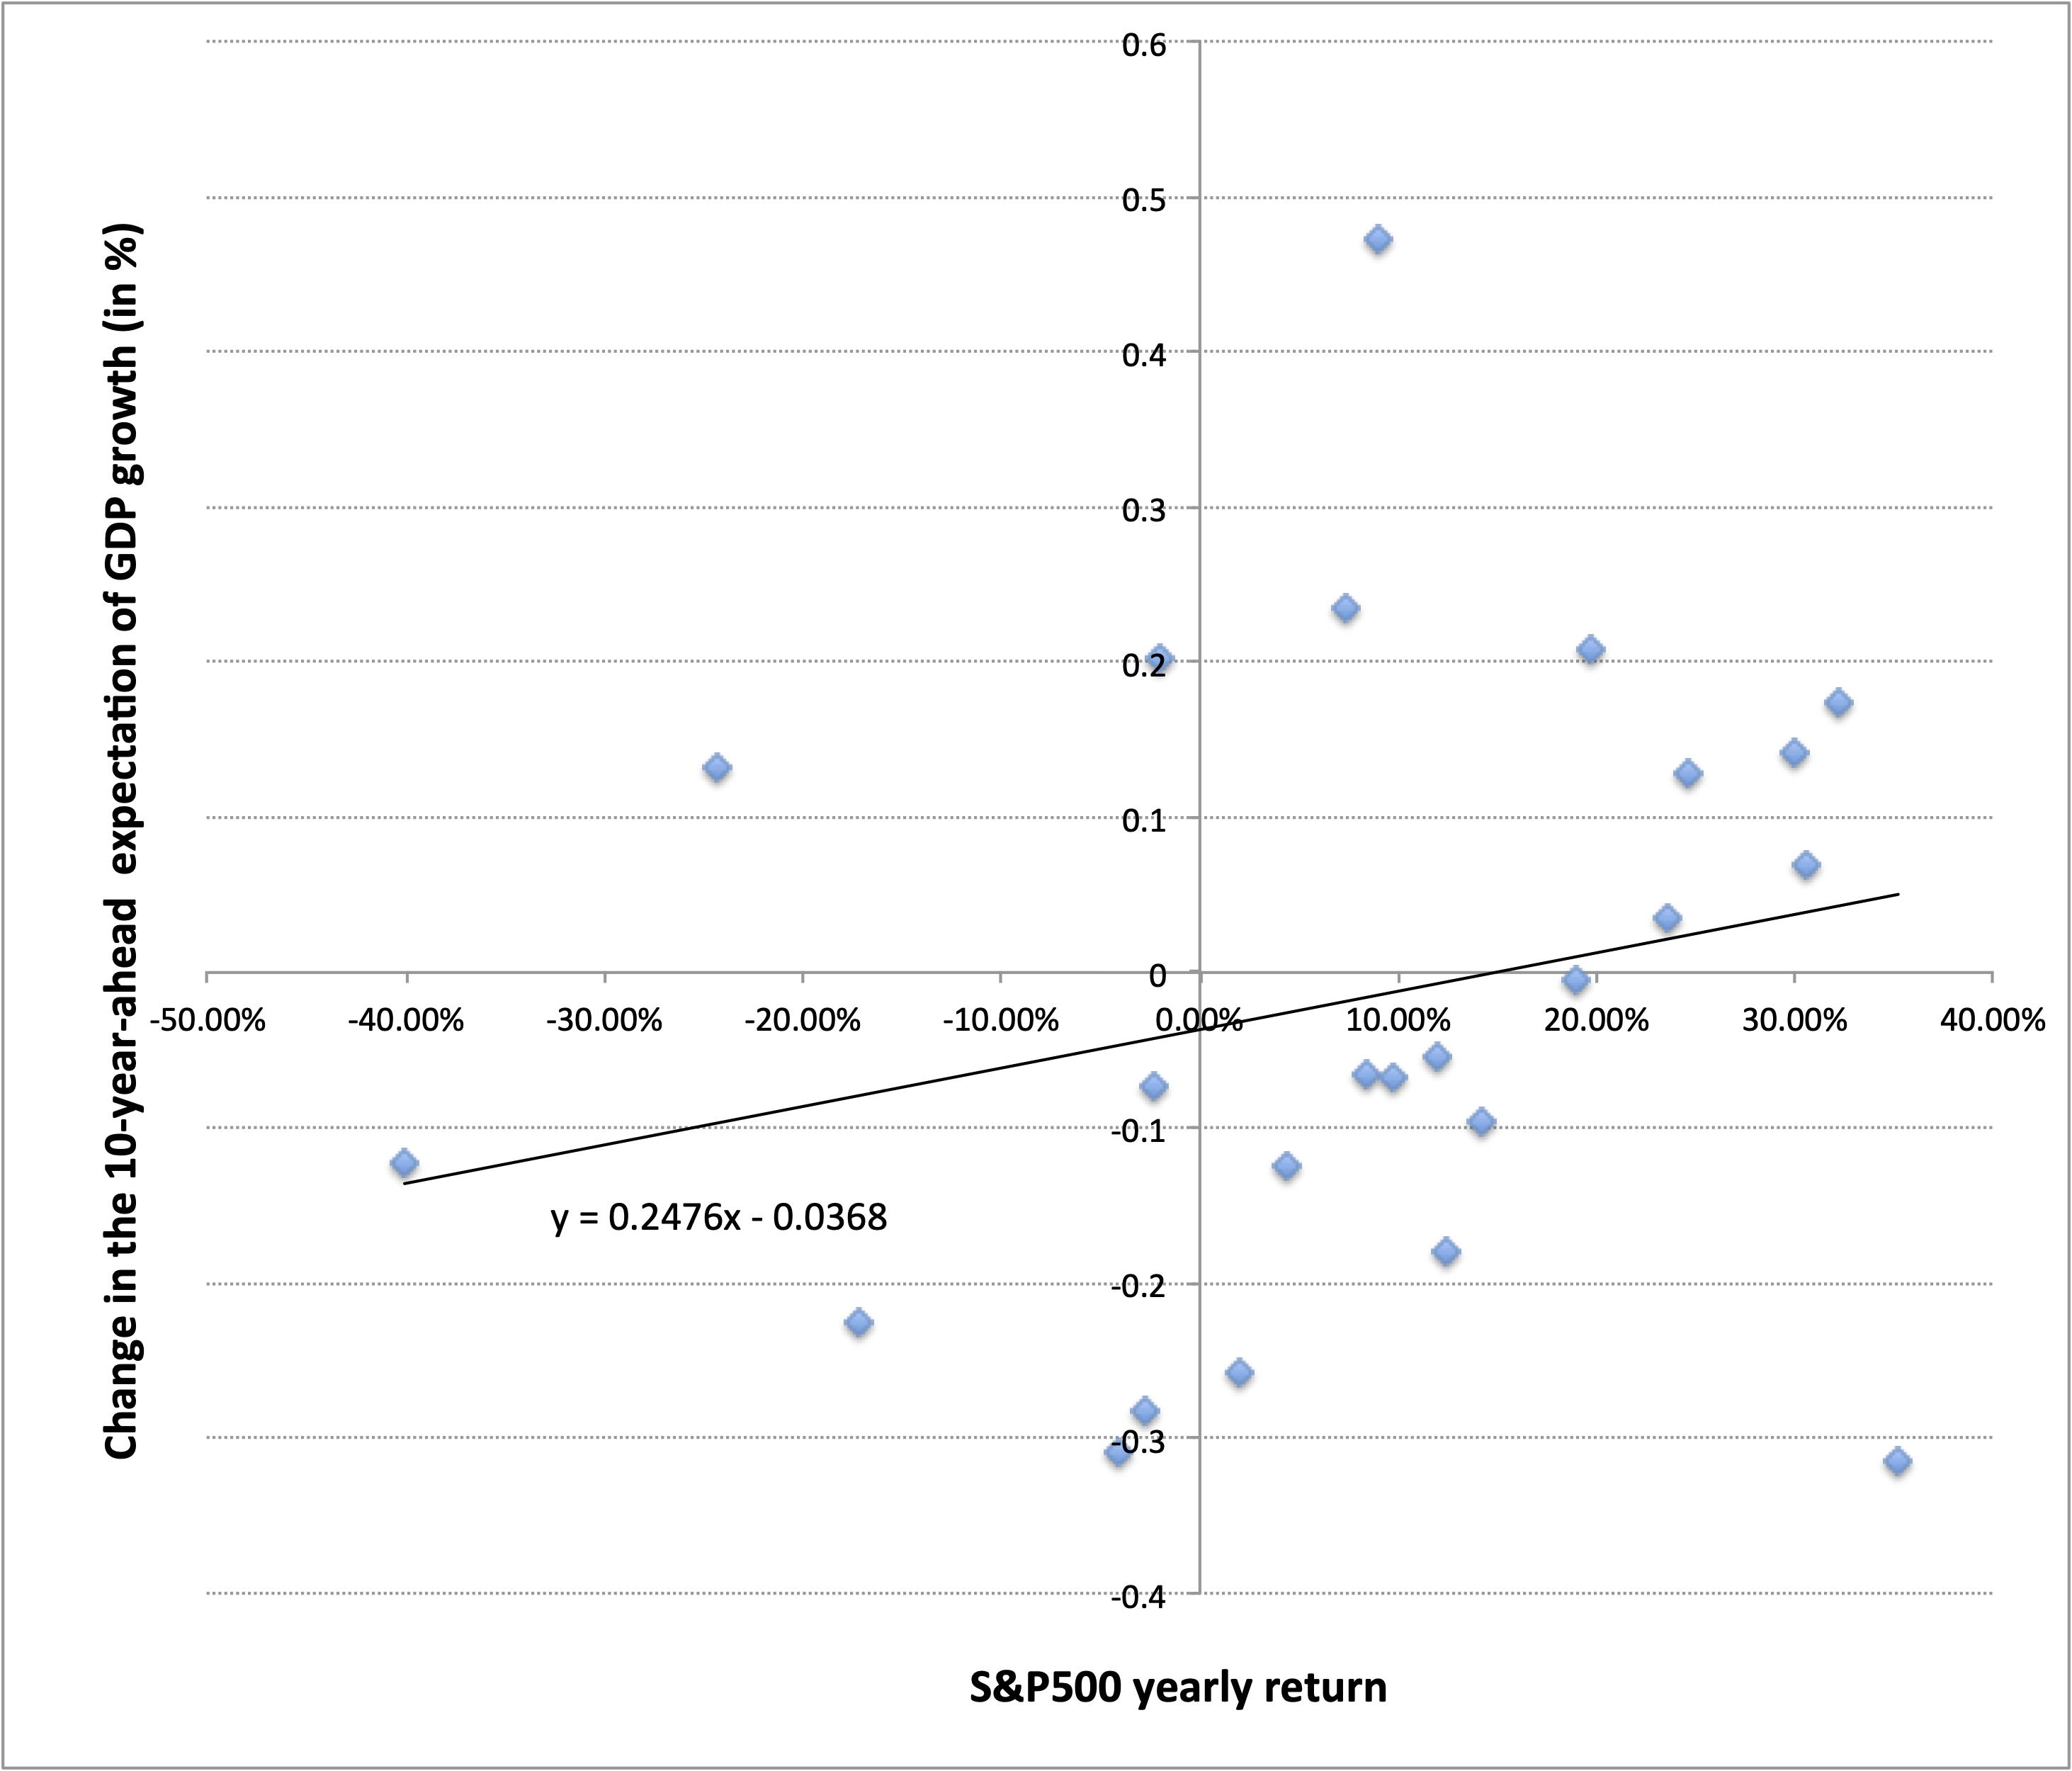
\includegraphics[width=1\linewidth]{figures/Figure_Stock_chge_expect} 

}

\caption{Source: Survey of Professional Forecasters (Philadelphia Fed).}\label{fig:SPF10yrStock}
\end{figure}

\hypertarget{long-run-risk-model}{%
\subsection{Long Run Risk Model}\label{long-run-risk-model}}

In this section, we present the model and approach proposed by \citet{Bansal_Yaron_2004}.
A \href{https://jrenne.shinyapps.io/LRRModels}{web interface} present outputs of the approach. It also allows to simulate the model dynamics and to assess the influence of the parameterization. \citet{Bansal_Yaron_2004} have proposed two models: an homoskedastic one and an heteroskedastic one. Three risk sources in the aggregate consumption dynamics:

\begin{itemize}
\tightlist
\item
  Short-run risk risks in consumption (high frequency),
\item
  Long-run risk risks in consumption (low frequency),
\item
  Fluctuations in consumption uncertainty (heteroskedastic model).
\end{itemize}

Another key ingredient: Epstein-Zin preferences.

Let's begin with the homoskedastic model.

\textbf{Bansal and Yaron (2004), homoskedastic}

\citet{Bansal_Yaron_2004} postulate the following dynamics for the economy:
\begin{eqnarray*}
x_{t+1} &=& \rho_x x_t + \phi_e \sigma e_{t+1}\\
\Delta c_{t+1} = g_{t+1} &=& \mu + x_t + \sigma \eta_{t+1}\\
g_{d,t+1} &=& \mu_d + \phi x_t + \phi_d \sigma u_{t+1},
\end{eqnarray*}
where \(e_{t+1},\eta_{t+1},u_{t+1} \sim i.i.d. \mathcal{N}(0,1)\).
\(\mu + x_t\): conditional expectation of consumption growth (\(g_t\));

\(g_{d,t}\): dividend growth rate (\(\log(D_{t+1}/D_t)\)).
Processes \(g_t\) and \(g_{d,t}\) are exogenous. The model is solved by finding associated processes \(r_{a,t}\) and \(r_{m,t}\) that make the model internally consistent:
These returns have to satisfy both Eqs. \eqref{eq:approxRa} and \eqref{eq:sdfRa}.
\(z_t\) and \(z_{m,t}\) are the log price-consumption and price-dividend ratios, respectively, i.e.:
\[
z_t = \log\left(\frac{P_{a,t}}{C_t}\right) \quad and \quad z_{m,t} = \log\left(\frac{P_{m,t}}{C_t}\right).
\]
\%(Eq. \eqref{eq:sdfRi} with \(r_{i,t}=r_{m,t}\) for \(z_{m,t}\))
The price of a claim on aggregate consumption is not observable (return: \(R_{a,t}\)), contrary to the price of the market portfolio (return: \(R_{m,t}\)).

Approach:

\begin{itemize}
\tightlist
\item
  Posit that \(z_t = A_0 + A_1 x_t\);
\item
  substitute the last expression into Eq. \eqref{eq:approxRa} and
\item
  inject \(r_{a,t+1}\) in Eq. \eqref{eq:sdfRa}.
\end{itemize}

This yields to:
\begin{equation}
A_1 = \frac{1- \dfrac{1}{\psi}}{1 - \kappa_1 \rho_x} \quad and \quad A_{1,m} = \frac{\Phi- \dfrac{1}{\psi}}{1 - \kappa_{1,m} \rho_x}.\label{eq:solABY1}
\end{equation}
If the IES \(\psi > 1\), then \(A_1 > 0\). The price-consumption ratio increases with long-term growth.
In this context, we have (from Eq. \eqref{eq:sdfEZ}):
\begin{eqnarray}
m_{t,t+1} - \mathbb{E}_t(m_{t,t+1}) &=& \left[  - \frac{\theta}{\psi} + \theta - 1\right] \sigma \eta_{t+1} \nonumber\\
&&- (1 - \theta)\left[ \kappa_1 \left( 1 - \frac{1}{\psi}\right) \frac{\phi_e}{1 - \kappa_1 \rho_x} \right]\sigma e_{t+1}\nonumber\\
&=& \lambda_{\eta} \sigma \eta_{t+1} - \lambda_{e} \sigma e_{t+1}.\label{eq:mBY1}
\end{eqnarray}
(Note that \(\lambda_{\eta} = -\gamma\).)
The higher \(\rho_x\), the higher \(\lambda_{e}\).

Consider any asset whose return is \(r_{i,t}\), that is: \(P_{i,t+1} = \exp(r_{i,t+1})P_{i,t}\). We must have:
\[
P_{i,t} = \mathbb{E}_t(\exp(m_{t,t+1})P_{i,t+1})= \mathbb{E}_t(\exp(m_{t,t+1}+r_{i,t+1})).
\]
Because the dynamics of the state vector is conditionally Gaussian, \(m_{t,t+1}+r_{i,t+1}\) is conditionally Gaussian. Hence:
\begin{eqnarray*}
1&=&\mathbb{E}_t\left(e^{m_{t,t+1}+r_{i,t+1}}\right)\\
&=&  \exp\left(\mathbb{E}_t(m_{t,t+1}+r_{i,t+1}) + \frac{1}{2}\mathbb{V}ar_t(m_{t,t+1}+r_{i,t+1})\right)\\
&=&  \exp\left(-r_{f,t}+\mathbb{E}_t(r_{i,t+1}) + \mathbb{C}ov_t(m_{t,t+1},r_{i,t+1}) + \frac{1}{2}\mathbb{V}ar_t(r_{i,t+1})\right).
\end{eqnarray*}
Therefore (particular case of Eq. \eqref{eq:MRCov}):
\begin{equation}
\mathbb{E}_t(r_{i,t+1}) -r_{f,t} = - \mathbb{C}ov_t(m_{t,t+1},r_{i,t+1}) - \frac{1}{2}\mathbb{V}ar_t(r_{i,t+1}).\label{eq:rpcond}
\end{equation}
The risk premium results from the conditional covariance between \(m_{t,t+1}\) and \(r_{i,t+1}\), i.e.~by the covariance of their innovations \(m_{t,t+1} - \mathbb{E}_t(m_{t,t+1})\) and \(r_{i,t+1} - \mathbb{E}_t(r_{i,t+1})\).

\begin{quote}
\textbf{About the solution procedure}. Eq. \eqref{eq:solABY1} shows that the \(A_i\)s depends on the \(\kappa_i\)s. Eq. \eqref{eq:approxRa} shows that the \(\kappa_i\)s depend on \(\bar{z}\).
Hence, in particular, \(A_0 = f(\bar{z})\). But, in turn, since \(z_t = A_0 + A_1 x_t\), we have \(\bar{z}=A_0 + A_1 \bar{x}=A_0\). For the model to be internally consistent, we should have \(\bar{z}=f(\bar{z})\). Hence, there is a fixed-point problem (\(\bar{z}\) cannot be chosen arbitrarily).
\end{quote}

\begin{example}[Prices of risk]
\protect\hypertarget{exm:PrRiskEZ}{}\label{exm:PrRiskEZ}Let us consider an asset whose log return is \(\beta\sigma\eta_{t+1}\) at date \(t+1\), i.e.~\(r_{i,t+1}=\beta\sigma\eta_{t+1}\).
Then Eq. \eqref{eq:rpcond} gives:
\[
\mathbb{E}_t(r_{i,t+1}) -r_{f,t} + \frac{1}{2}\beta^2\sigma^2 = - \lambda_{\eta}\beta\sigma^2.
\]
Because \(\lambda_{\eta}=-\gamma<0\), \$ - \lambda\_\{\eta\}\beta\sigma\^{}2\$ is positive if \(\beta\ge0\).
\(\lambda_\eta\) (resp. \(\lambda_{e}\)) measures the price of the ``\(\eta\) risk'' (resp. the ``\(e\) risk'').
\(\beta\) measures the exposure of stock \(i\) to the shock \(\eta_{t}\).
\end{example}

Exploiting Eqs. \eqref{eq:approxRa} (for \(r_{m,t}\)), \eqref{eq:solABY1} and the model dynamics, we get:
\begin{equation}
r_{m,t+1} - \mathbb{E}_t(r_{m,t+1}) = \phi_d  \underbrace{\sigma u_{t+1}}_{\mbox{not "priced"}} + \beta_{m,e}  \underbrace{ \sigma e_{t+1}}_{\mbox{"priced"}},\label{eq:rmErm}
\end{equation}
where \(\beta_{m,e} = \kappa_{1,m}\left(\phi - \dfrac{1}{\psi}\right)\dfrac{\phi_e}{1 - \kappa_{1,m} \rho_x}\).
Then, using Eq. \eqref{eq:mBY1}, Eq. \eqref{eq:rpcond} gives, for \(r_{i,t+1}=r_{m,t+1}\):
\begin{equation}
\mathbb{E}_t(r_{m,t+1} - r_{f,t}) = \beta_{m,e}\lambda_{e} \sigma^2 - 0.5 \mathbb{V}ar_t(r_{m,t}),\label{eq:xsBYhomo}
\end{equation}
where, by Eq. \eqref{eq:rmErm}, we have \(\quad\mathbb{V}ar_t(r_{m,t})=(\beta_{m,e}^2+\phi_d^2)\sigma^2\).
\(\beta_{m,e}\) measure the exposure of stocks to the long-run risk shock \(e_t\).
The risk premium increases with \(\rho_x\). Similarly, BY show that the volatility of the market return increases with \(\rho_x\). \href{https://jrenne.shinyapps.io/LRRModels}{web interface}.

\textbf{Remnark}: constant \(\sigma\) \(\Rightarrow\) constant risk premium.

\textbf{Bansal and Yaron (2004), heteroskedastic}

\citet{Bansal_Yaron_2004} then introduce conditional volatility in the model:
\begin{eqnarray}
x_{t+1} &=& \rho_x x_t + \phi_e \sigma_t e_{t+1} \nonumber\\
g_{t+1} &=& \mu + x_t + \sigma_t \eta_{t+1} \nonumber\\
g_{d,t+1} &=& \mu_d + \phi x_t + \phi_d \sigma_t u_{t+1} \nonumber\\
\sigma_{t+1}^2 &=& \sigma^2 + \nu_1(\sigma^2_t -\sigma^2) + \sigma_w w_{t+1}, \label{eq:BYheteroscked}
\end{eqnarray}
where \(e_{t+1},\eta_{t+1},u_{t+1},w_{t+1} \sim i.i.d. \mathcal{N}(0,1)\).
Here, the posited solution for \(z_t\) is:
\[
z_t = A_0 + A_1 x_t + {\color{red}A_2 \sigma^2_t}.
\]
\(A_1\) is unchanged. \(A_2\) is given by (similar form for \(A_{2,m}\)):
\[
A_2 = \frac{0.5 \left[ \left(\theta - \dfrac{\theta}{\psi}\right)^2 + (\theta A_1 \kappa_1 \phi_e)^2 \right]}{\theta(1 - \kappa_1 \nu_1)}.
\]
Remark ??? also applies in this context.

The innovation of the SDF is:
\begin{eqnarray}
m_{t,t+1} - \mathbb{E}_t(m_{t,t+1}) = \lambda_{\eta} \sigma_t \eta_{t+1} - \lambda_{e} \sigma_t e_{t+1} - \lambda_{w} \sigma_w w_{t+1},\label{eq:mBY2}
\end{eqnarray}
where \$ \lambda\_\{w\} = (1-\theta)A\_2 \kappa\_1\$ and \(\lambda_e\) and \(\lambda_\eta\) are as in Eq. \eqref{eq:sdfEZ}.
In the case of power utility (\(\theta = 1\)), the third term vanishes.
The innovation of the market return is:
\begin{equation}
r_{m,t+1} - \mathbb{E}_t(r_{m,t+1}) = \phi_d  \underbrace{\sigma_t u_{t+1}}_{\mbox{not "priced"}} + \beta_{m,e}  \underbrace{ \sigma_t e_{t+1}}_{\mbox{"priced"}} + \beta_{m,w}  \underbrace{ \sigma_w w_{t+1}}_{\mbox{"priced"}}.\label{eq:rmErmHetero}
\end{equation}
Then Eq. \eqref{eq:rpcond} gives, for \(r_{i,t+1}=r_{m,t+1}\):
\begin{equation}
\mathbb{E}_t(r_{m,t+1} - r_{f,t}) = \beta_{m,e}\lambda_{e} \sigma_t^2 + \beta_{m,w}\lambda_{w} \sigma_t^2 - 0.5 \mathbb{V}ar_t(r_{m,t}).\label{eq:xsBYhetero}
\end{equation}
Increase in volatility \(\Rightarrow\) augments excess returns. But this does not reflect increases in dividends \(\Rightarrow\) equity prices decrease {[}Eq. \eqref{eq:dp2}{]}.

Increase in uncertainty \(\Rightarrow\) Decrease in prices.

Compared the homoskedastic case {[}Eq. \eqref{eq:xsBYhomo}{]}, (a) the expected excess return is time-varying and (b) additional term = compensation for stochastic volatility risk in consumption.

ratio of conditional risk premium to the conditional volatility of the market portfolio is time-varying (TV) \(\Rightarrow\) TV Sharpe ratio.
Maximal Sharpe ratio \(\approx\) conditional volatility of the SDF innovations. It is TV.

The same kind of computation can be carried out for the return of the consumption claim (\(r_{a,t}\)). We get:
\begin{equation}
r_{a,t+1} - \mathbb{E}_t(r_{a,t+1}) = \sigma_t \eta_{t+1} + \beta_{a,e}  \sigma_t e_{t+1} + \beta_{a,w}  \sigma_w w_{t+1},\label{eq:raEraHetero}
\end{equation}
where \(\beta_{a,e}=\kappa_1 A_1 \phi_e\) and \(\beta_{a,w}=\kappa_1A_2\).
Eq. \eqref{eq:rpcond} then gives:
\begin{equation}
\mathbb{E}_t(r_{a,t+1} - r_{f,t}) = -\lambda_{\eta} \sigma_t^2 + \beta_{a,e}\lambda_{e} \sigma_t^2 + \beta_{a,w}\lambda_{w} \sigma_t^2 - 0.5 \mathbb{V}ar_t(r_{a,t}).\label{eq:xsaBYhetero}
\end{equation}

The short term rate \(r_{f,t}\) is such that \(\exp(-r_{f,t})=\mathbb{E}_t(\exp(m_{t,t+1}))\).
Using Eq. \eqref{eq:sdfEZ}, we get:
\[
\exp(-r_{f,t})=\mathbb{E}_t\left(\exp\left[\theta \log \delta - \frac{\theta}{\psi} g_{t+1} - (1-\theta) r_{a,t+1}\right]\right).
\]
We have:
\begin{equation}
r_{f,t} = - \theta \log (\delta) + \mathbb{E}_t\left(\frac{\theta}{\psi} g_{t+1}+ (1-\theta)r_{a,t+1} \right) - \frac{1}{2}\mathbb{V}ar_t\left(\frac{\theta}{\psi} g_{t+1} + (1-\theta) r_{a,t+1}\right),
\end{equation}
which, after computation, gives:
\begin{equation}
r_{f,t} = - \log (\delta) + \frac{1}{\psi}\mathbb{E}_t(g_{t+1})+ \frac{1-\theta}{\theta} \mathbb{E}_t(r_{a,t+1}-r_{f,t}) - \frac{1}{2\theta}\mathbb{V}ar_t\left(m_{t,t+1}\right),\label{eq:rfBY}
\end{equation}
where \(\mathbb{V}ar_t\left(m_{t,t+1}\right)\) is easily obtained from Eq. \eqref{eq:mBY2} and \(\mathbb{E}_t(r_{a,t+1}-r_{f,t})\) is given by Eq. \eqref{eq:xsaBYhetero}.

Regressing \(r_{f,t}\) on \(g_{t+1}\) may give an estimate of \(1/\psi\). BY: Time-varying intercept implies a downward bias on \(\hat\psi\).

The model-implied time-series properties are consistent with the data.

With persistent expected growth, the model is able to generate sizeable risk premiums, market volatility and fluctuations in price-dividend ratios {[}Slide XXX{]}.
Larger risk aversion increases the equity premium {[}Slide XXX{]}.
In order to match data features, the IES has to be \(>1\).

Lowering the IES reduces the elasticity of asset prices to dividends, namely \(A_{1,m}\) {[}Eq. \eqref{eq:solABY1}{]}, which reduces risk premia \href{https://jrenne.shinyapps.io/LRRModels}{web interface}.

If the IES is too small, this elasticity becomes negative: rise in dividend growth rate \(\Rightarrow\) decreases in prices.

Lower part of the table in Slide XXX: i.i.d. growth rates. Then no correlation between dividend growth and consumption, and \(\mathbb{E}_t(r_{m,t+1}-r_{f,t})=-1/2 \mathbb{V}ar_t(r_{m,t+1}) < 0\).

While the time series properties of the model with small persistent expected growth are difficult to distinguish from a pure i.i.d. model, its asset-pricing implications are drastically different.
Evidence in favor of the heteroskedastic model: In particular, relationship between the absolute values of innovations in consumption and the log price-dividend ratio (Table III in \citet{Bansal_Yaron_2004}).
Moments implied by the heteroskedastic model are shown in Table IV of \citet{Bansal_Yaron_2004}.
{[}\(\Rightarrow\){]} Good fit of the data first and second moments.
Volatility of the SDF: the persistency of the expected growth rate is key (divided by two when \(\rho_x\) is set to 0).
The model replicates the way price-dividend ratios predict excess returns {[}Slide XXX{]}.

\begin{figure}

{\centering 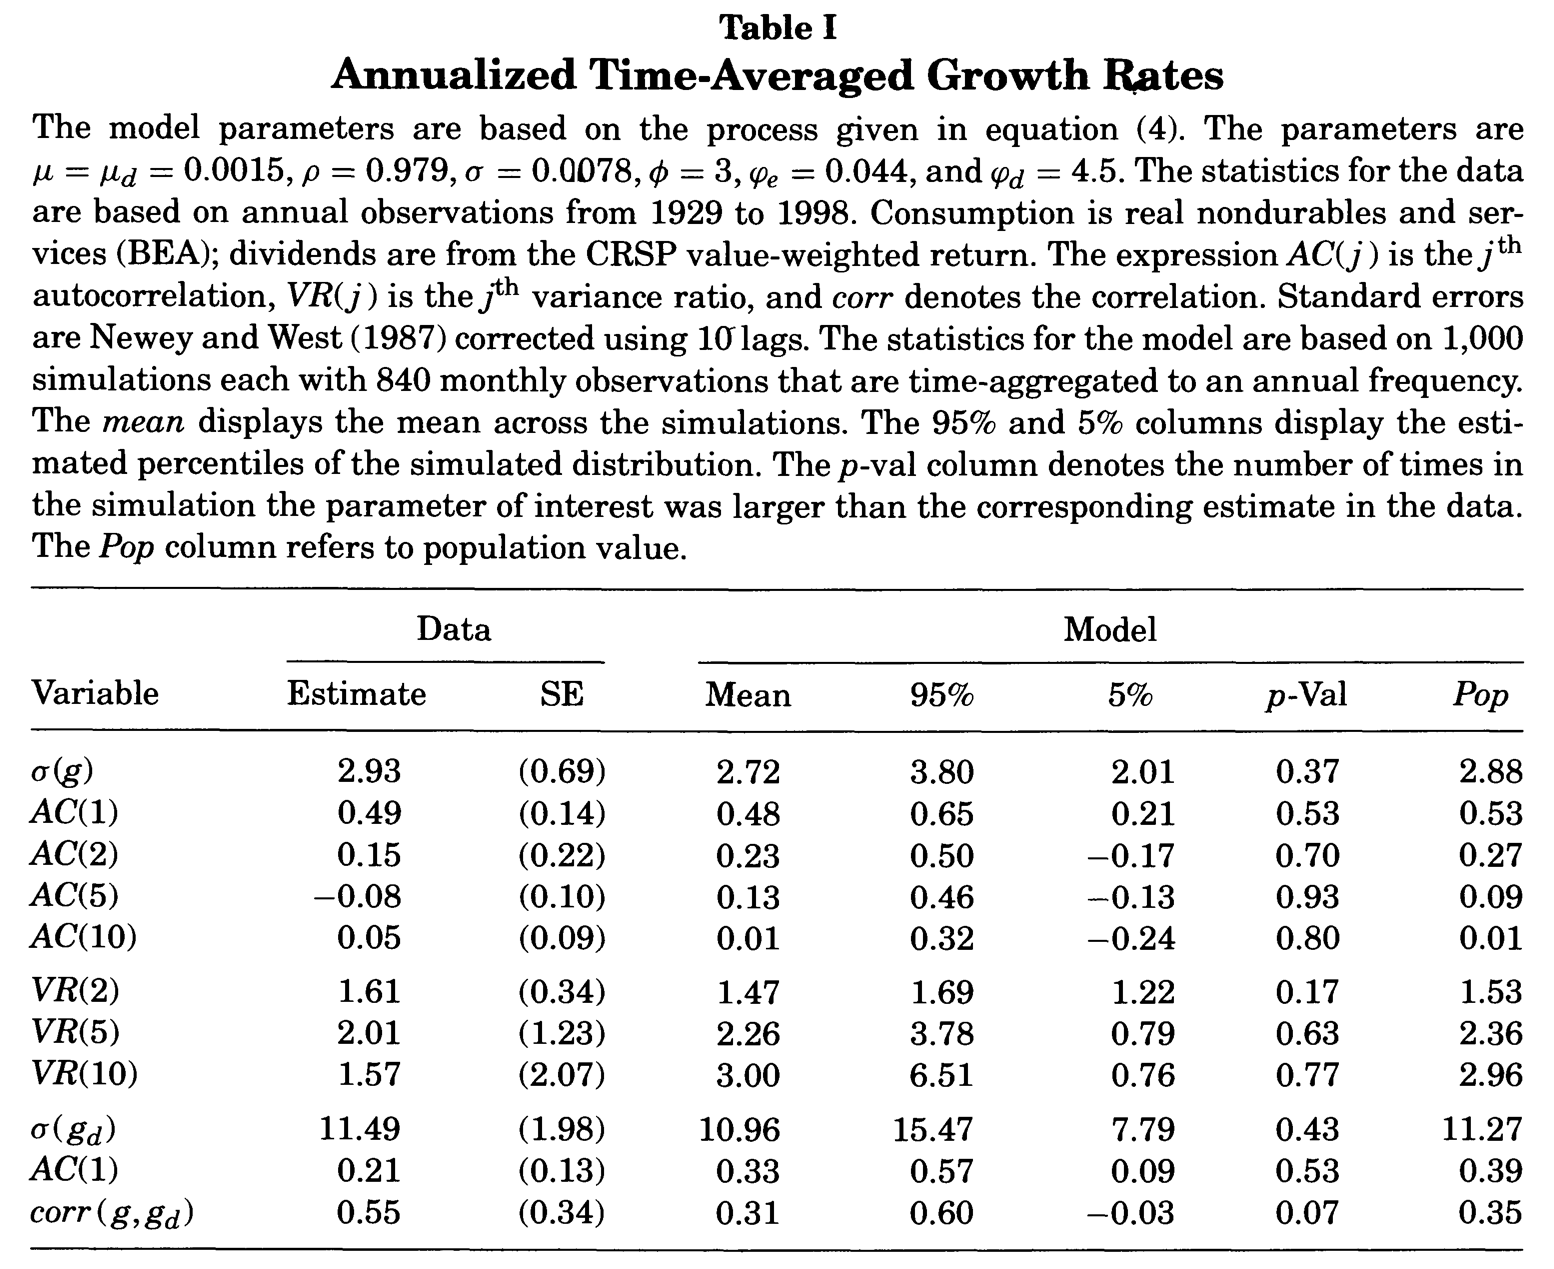
\includegraphics[width=1\linewidth]{figures/table_BY1} 

}

\caption{Source: Bansal and Yaron (2004).}\label{fig:BY1}
\end{figure}

\begin{figure}

{\centering 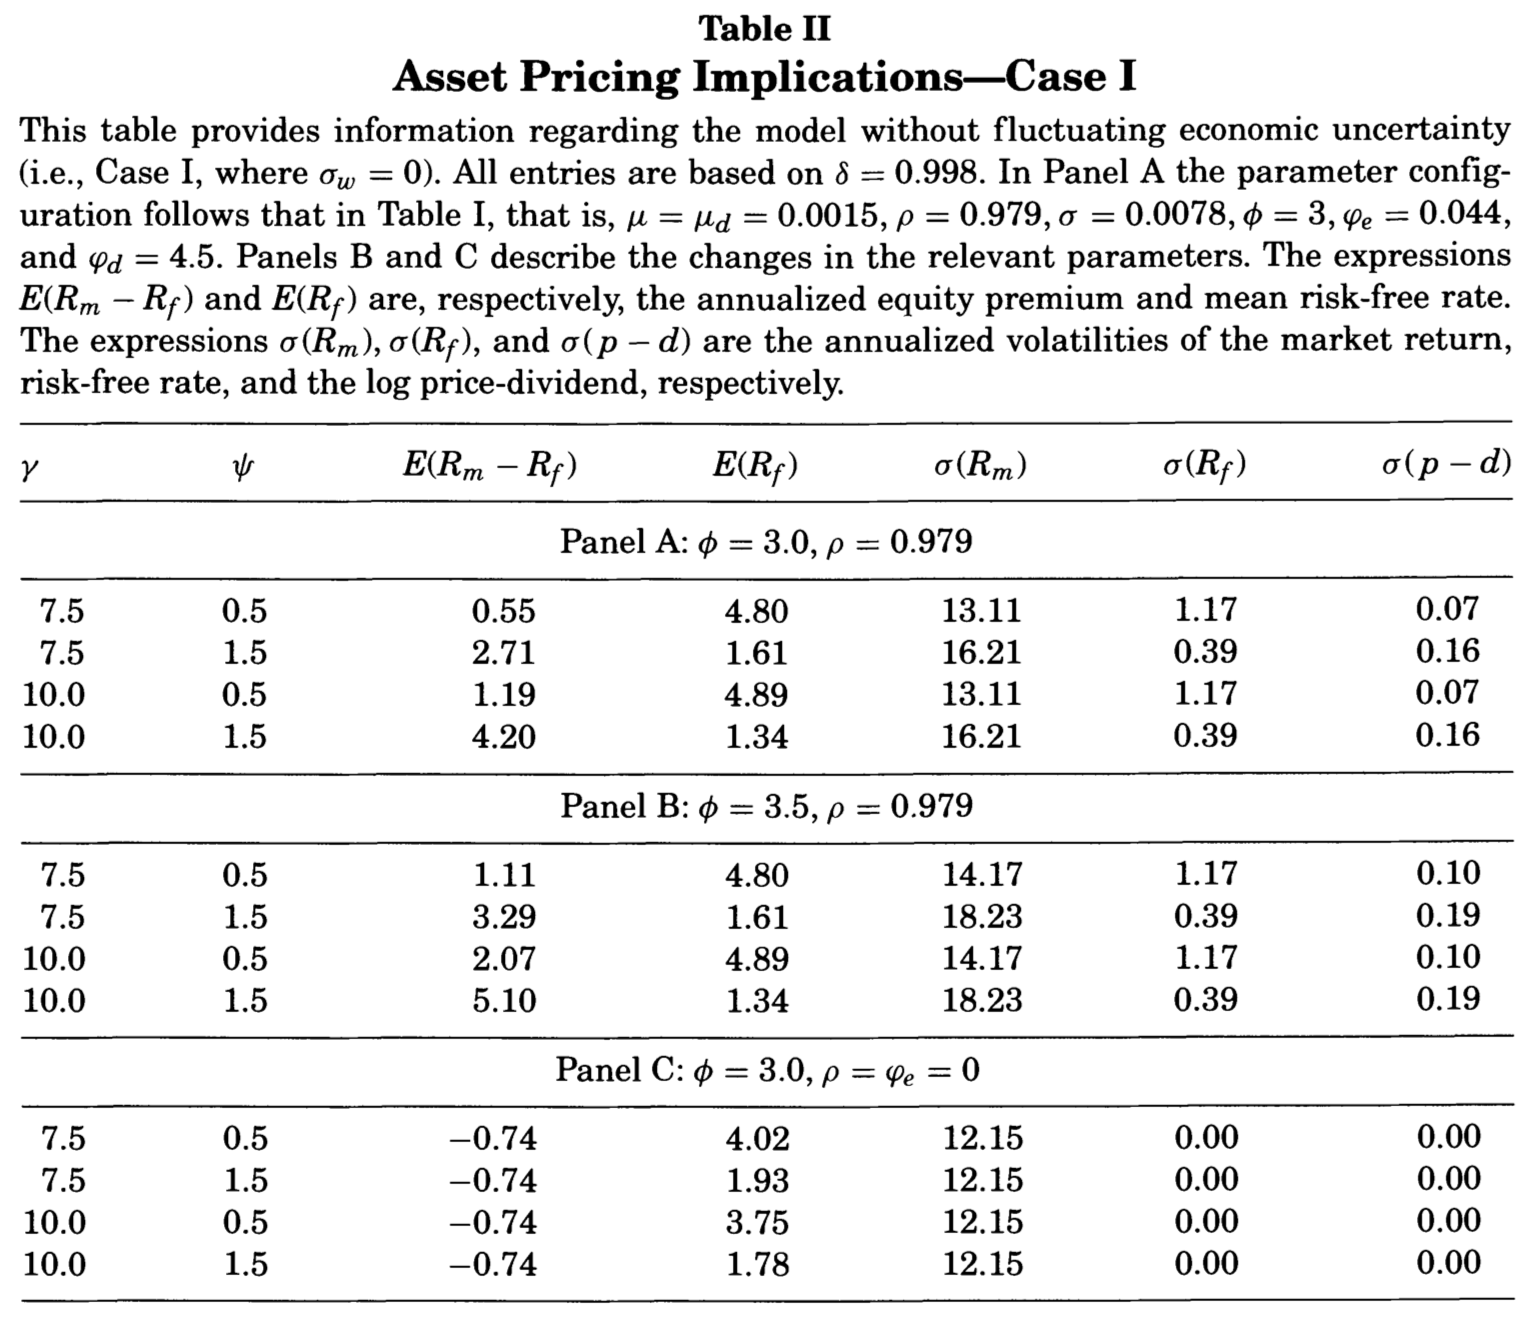
\includegraphics[width=1\linewidth]{figures/table_BY2} 

}

\caption{Source: Bansal and Yaron (2004).}\label{fig:BY2}
\end{figure}

\begin{figure}

{\centering 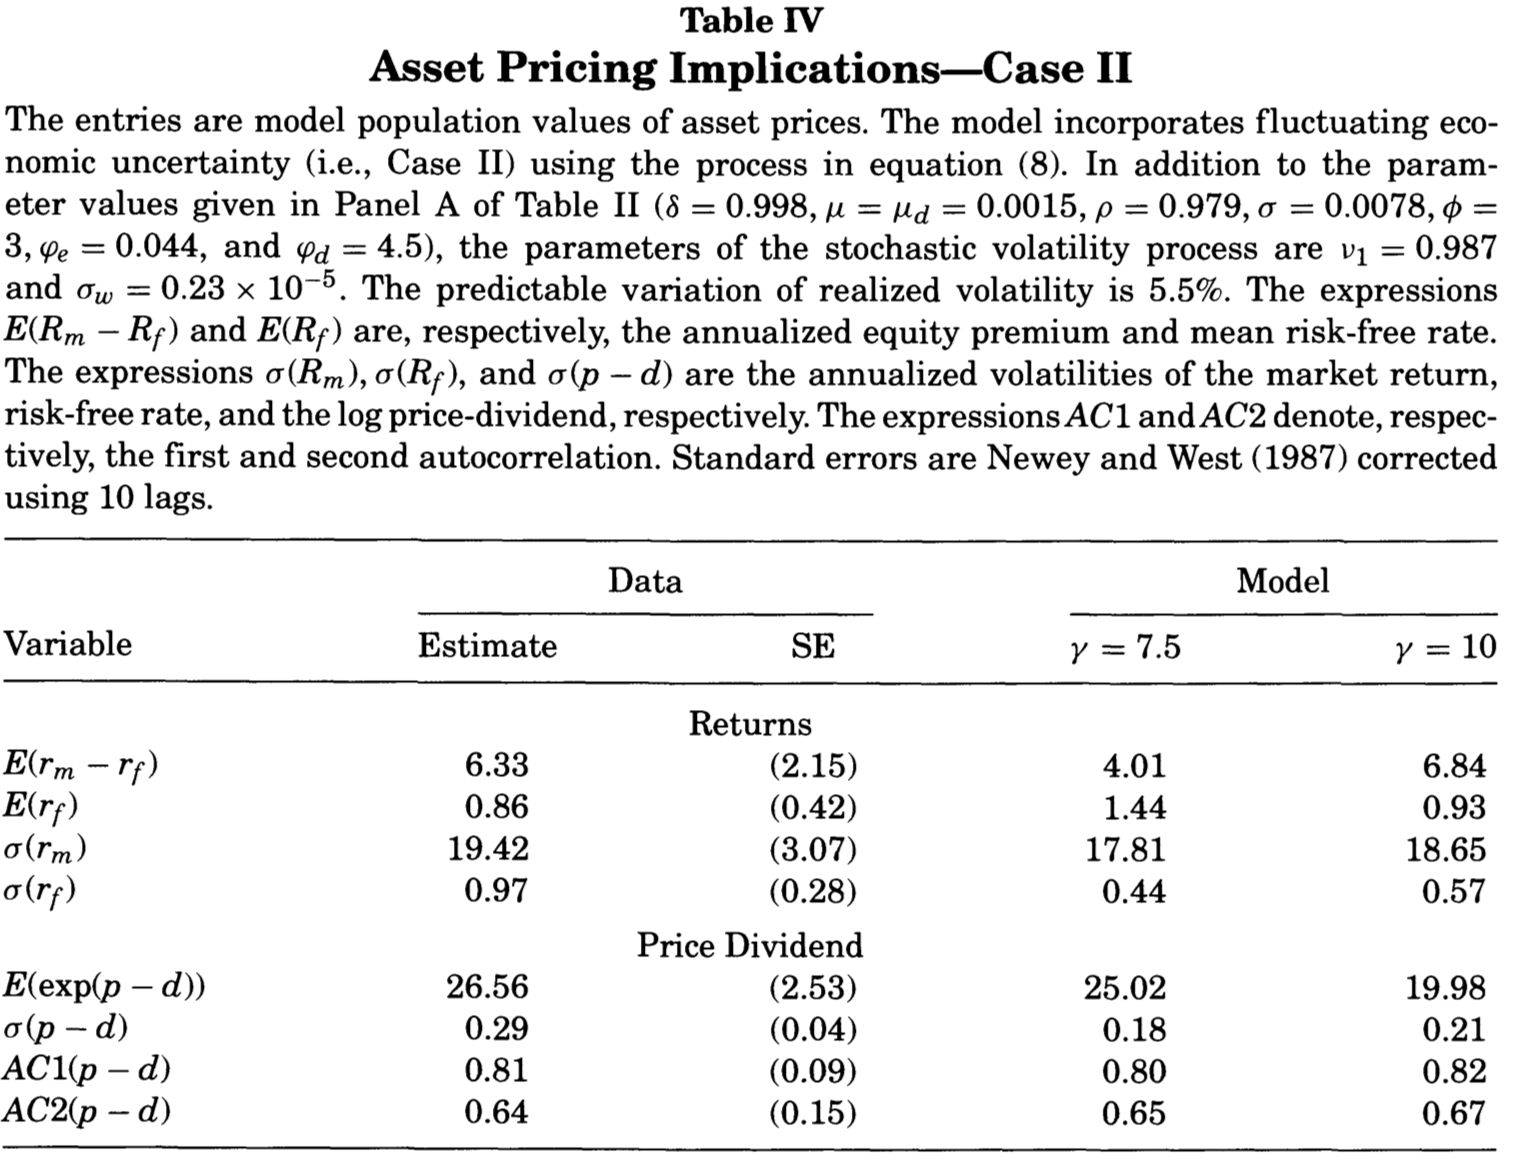
\includegraphics[width=1\linewidth]{figures/table_BY4} 

}

\caption{Source: Bansal and Yaron (2004).}\label{fig:BY3}
\end{figure}

\begin{figure}

{\centering 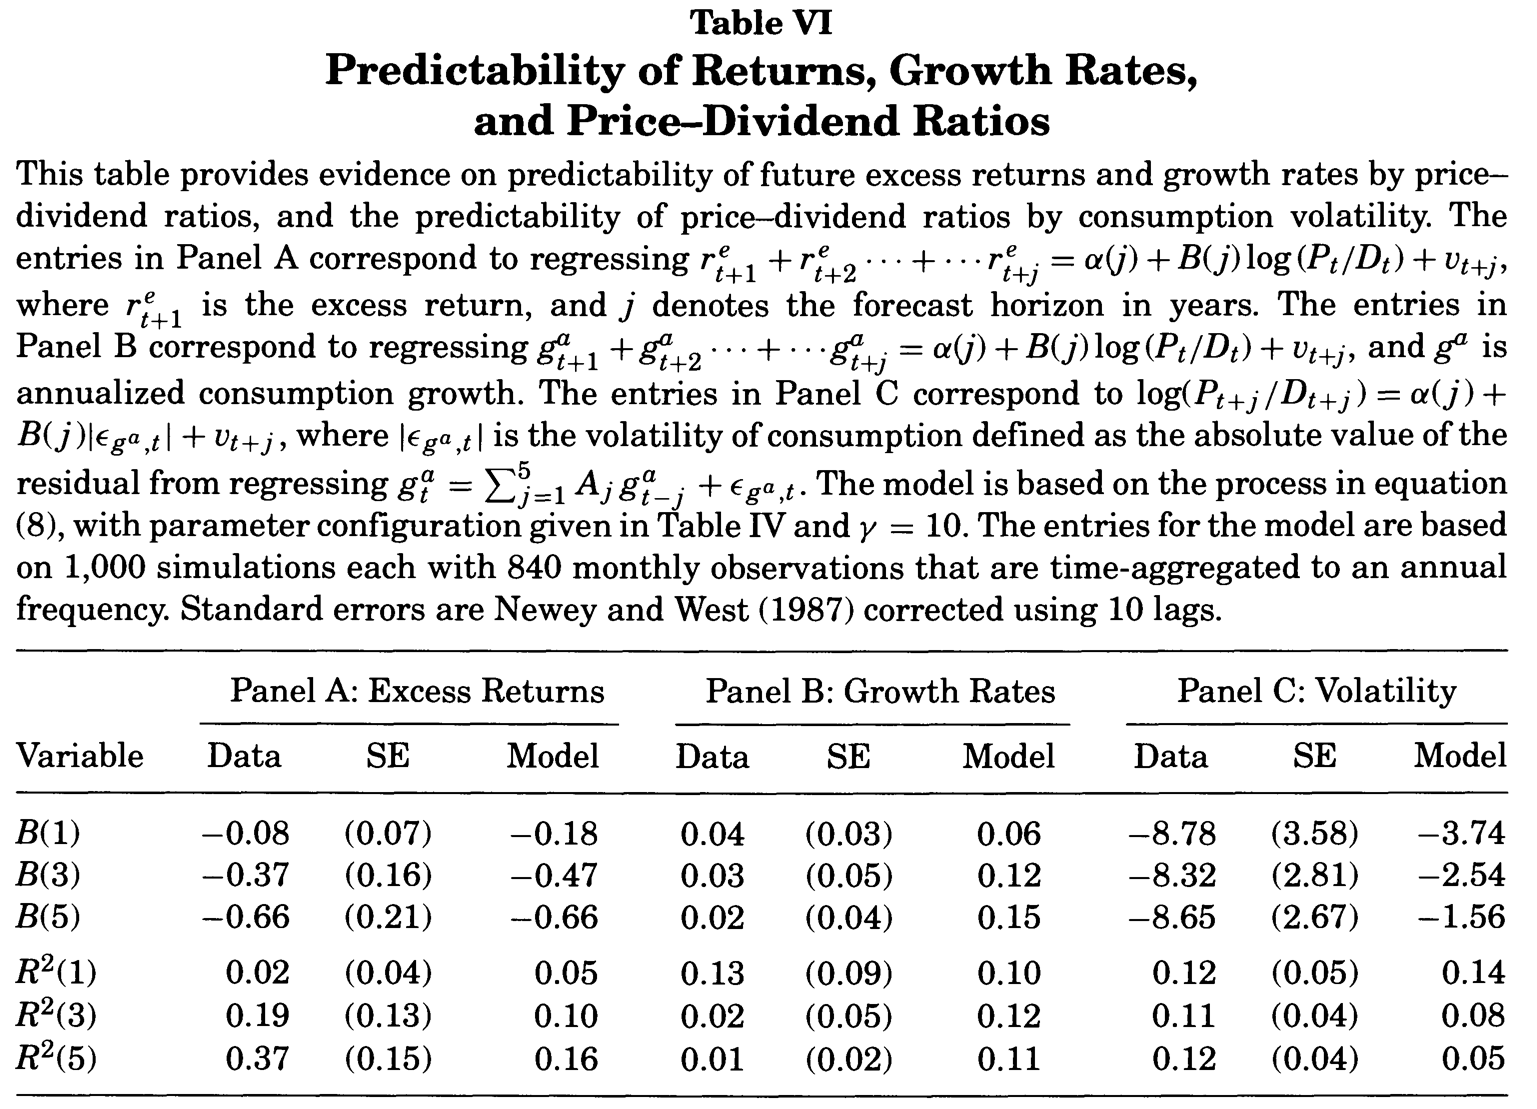
\includegraphics[width=1\linewidth]{figures/table_BY6} 

}

\caption{Source: Bansal and Yaron (2004).}\label{fig:BY4}
\end{figure}

\{Empirics of the LRR model: Bansal, Kiku and Yaron (2007)\}

\citet{Bansal_Kiku_Yaron_2016} show that their model is supported by cross-section data.
Specifically, they want to see whether their model is able to reproduce the differences in excess returns for small/large and value/growth stocks {[}Slide XXX{]}.
The model is slightly modified. The process followed by the dividend growth rate associated to stock \(i\) is:
\[
g^{(i)}_{d,t+1} = \mu_d^{(i)} + \phi^{(i)} x_t + \pi^{(i)}\sigma_t \eta_{t+1} +  \phi^{(i)} \sigma u_{i,t+1}.
\]
Therefore, in this model, stock prices are also exposed to the short-run consumption growth rate \(\eta_t\).

Starting point: \(r_{f,t}\) and \(z_{m,t}\) are observable.
Both variables are linear in \(X_t=[x_t,\sigma_t^2]'\) {[}SlideXXX\} for \(r_{f,t}\){]}.
Hence, if one regress \(\Delta c_{t+1}\) on \(Y_t=[r_{f,t},z_t]\), the residuals are the same as those obtained when regressing \(\Delta c_{t+1}\) on \(X_t\), i.e.~\(\sigma_t \eta_{t+1}\).

Besides, \(\mathbb{E}_t(\sigma_t^2 \eta_{t+1}^2)=\sigma_t^2\) is also a linear function of \(X_t\). Therefore, the fitted values in the regression of \(\sigma_t^2 \eta_{t+1}^2\) on \(X_t\) provide estimates of \(\sigma_t^2\).
Once we have estimates of \(x_t\) and \(\sigma^2_t\), one can easily get estimates of their respective innovations, \(e_t\) and \(w_t\).
For stock (or portfolio) \(i\), BKY regress \(r_{i,t+1}\) on \(Y_t\). This provide them with estimates of the expected returns \(\mathbb{E}_t(r_{i,t+1})\). The beta's of stock \(i\) are then measured as the covariances between \(r_{i,t+1}-\mathbb{E}_t(r_{i,t+1})\) and the estimates of the shocks \(\eta_t\), \(e_t\) and \(w_t\) (divided by the variance of these shocks).
100 Fama-French porfolio (10 sizes and 10 book-to-market values); average excess returns are regressed on the beta's.
{[}\(\Rightarrow\){]} The three beta's explain about 84\% of the cross-sectional variation in mean returns.
Macroeconomic interpretation of the Fama-French pricing factors (change of basis).

\begin{figure}

{\centering 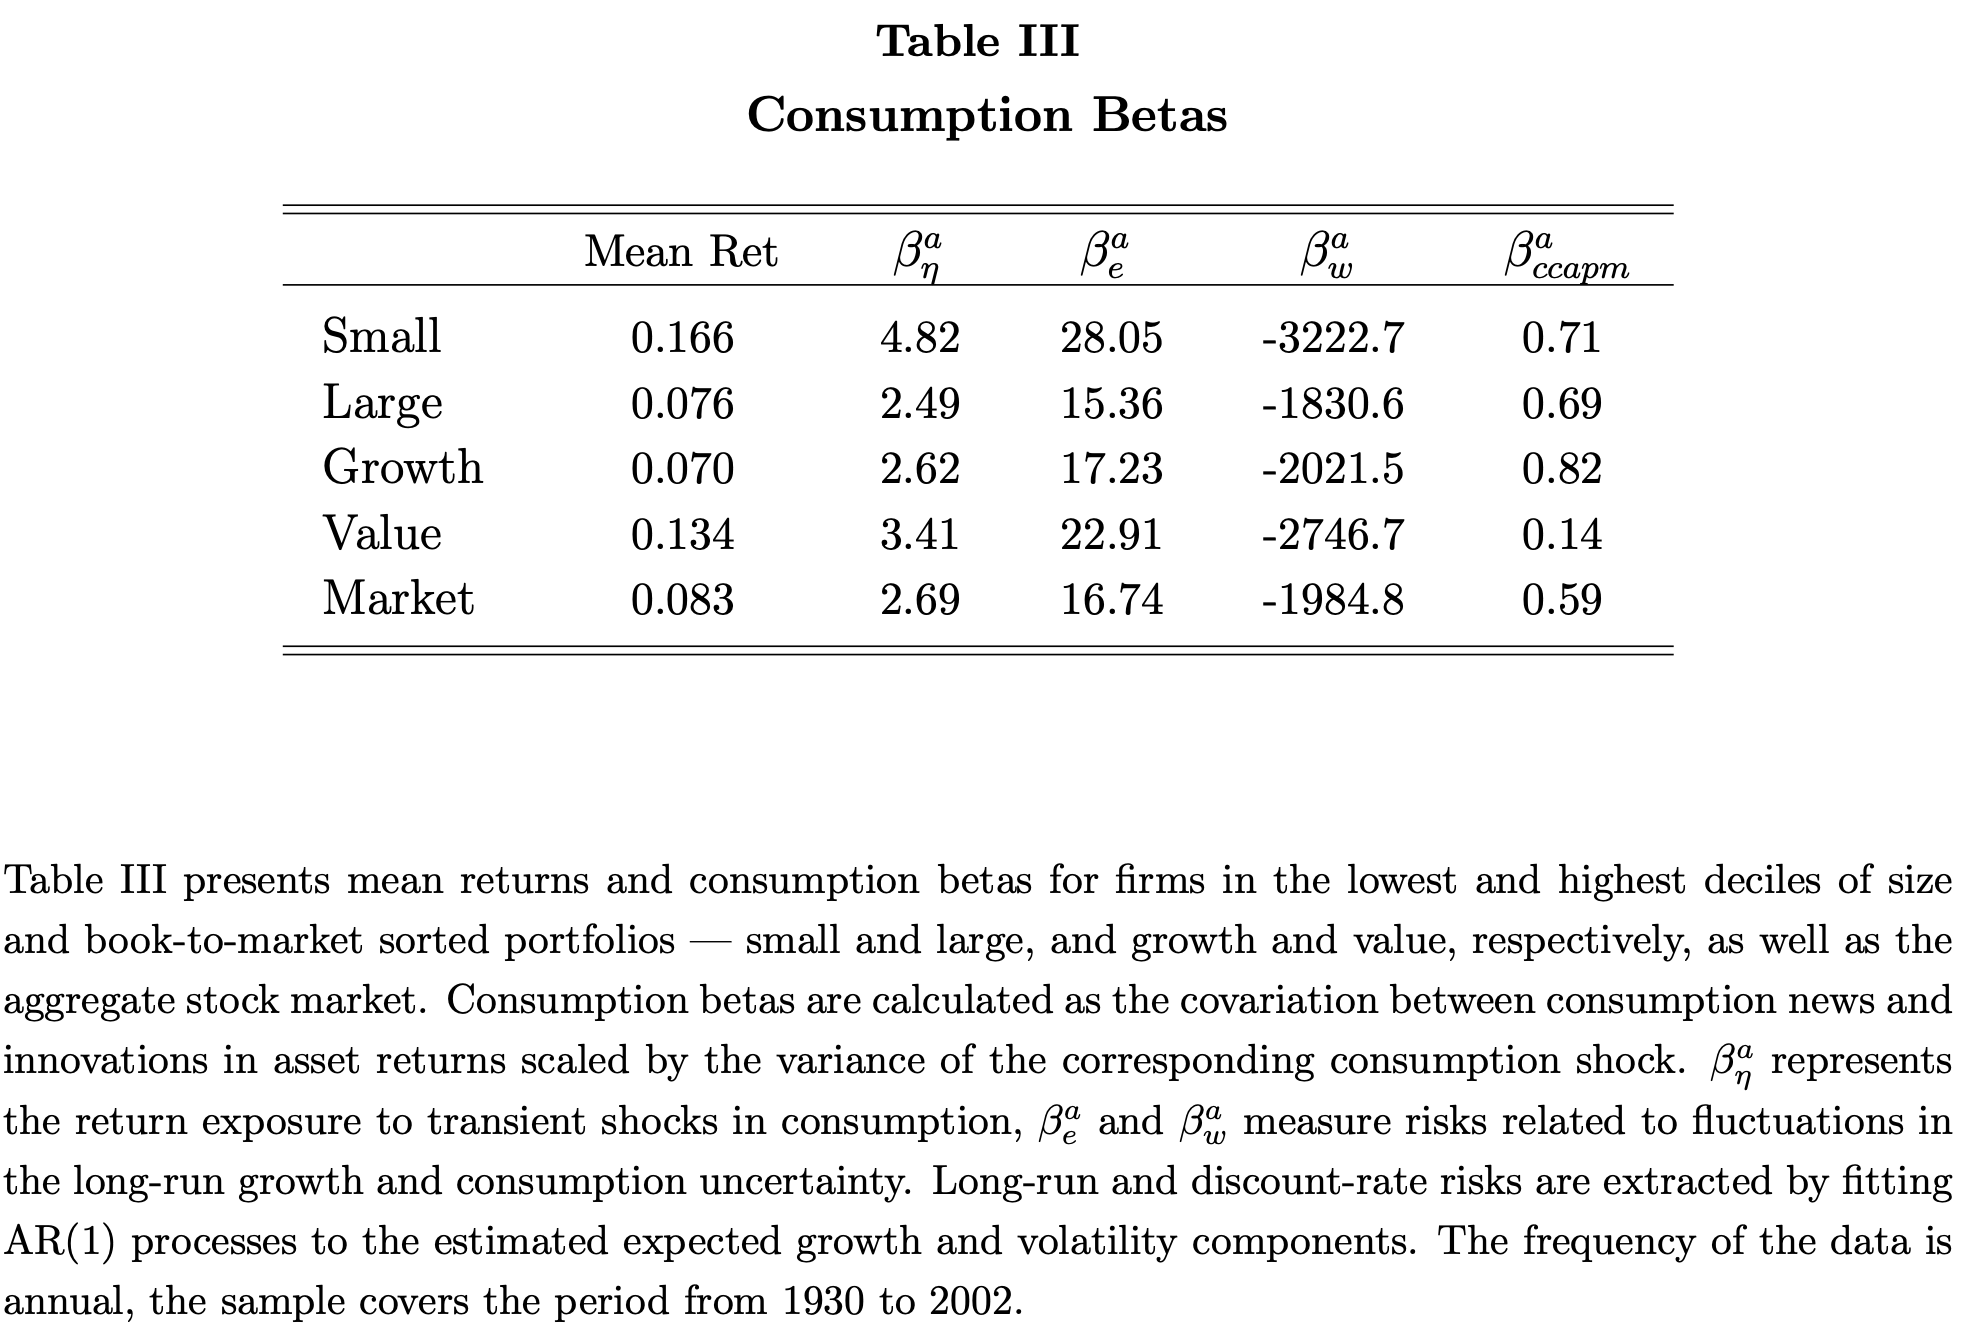
\includegraphics[width=1\linewidth]{figures/table_BKY1} 

}

\caption{Source: Bansal, Kiku, and Yaron (2016).}\label{fig:BKY1}
\end{figure}

\begin{figure}

{\centering 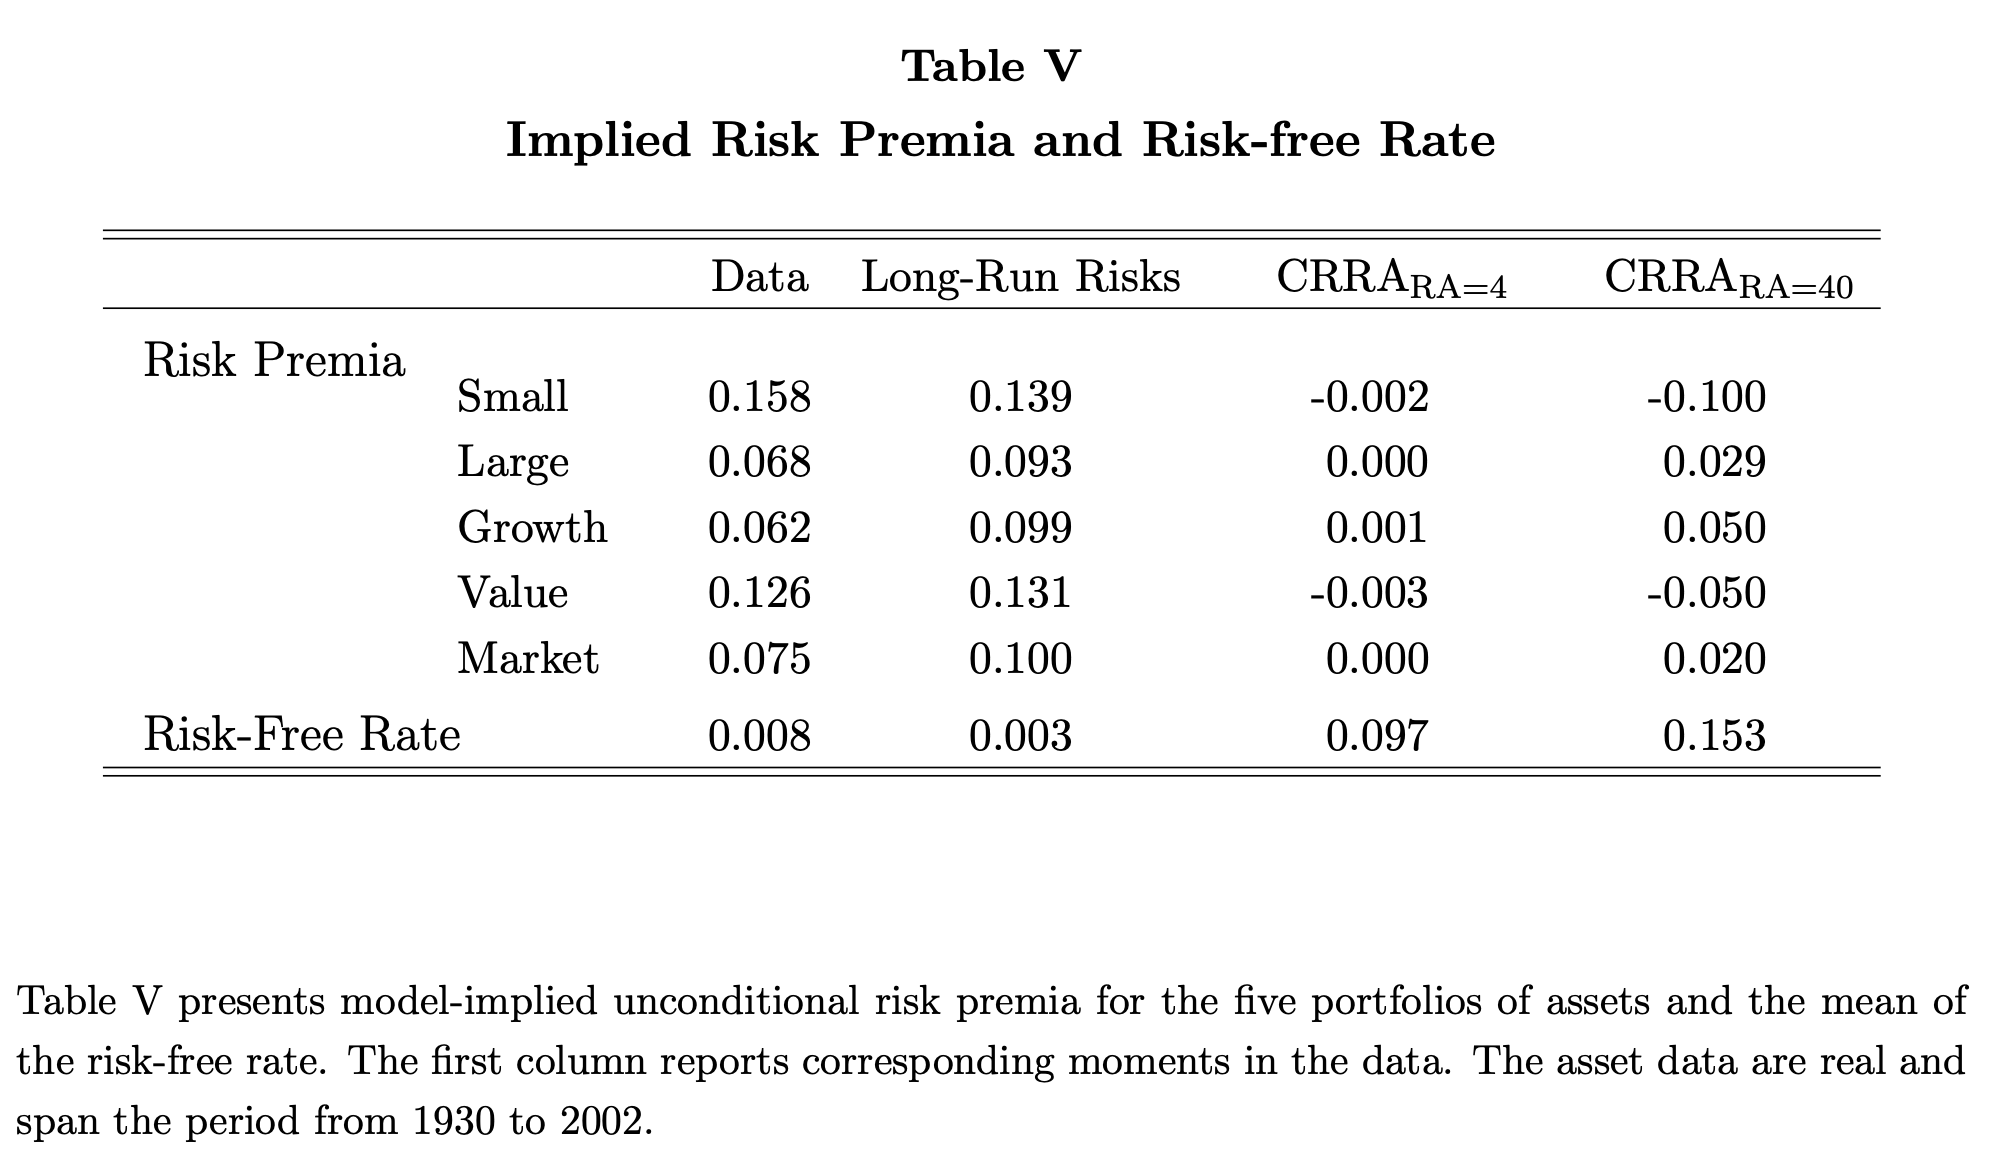
\includegraphics[width=1\linewidth]{figures/table_BKY2} 

}

\caption{Source: Bansal, Kiku, and Yaron (2016).}\label{fig:BKY2}
\end{figure}

\hypertarget{appendix}{%
\section{Appendix}\label{appendix}}

\hypertarget{SDFEZ}{%
\subsection{SDF in the CES Epstein-Zin Context}\label{SDFEZ}}

We denote by \(\pi_t(x_{t+1})\) the price of an asset that provides the payoff \(x_{t+1}\) at date \(t+1\) (as of date \(t\), this payoff may be random). If one purchases \(\varepsilon\) units of this asset and consumes them at date \(t+1\), the intertemporal utility becomes \(F(C_t\color{blue}{ - \varepsilon \pi_t(x_{t+1})},R_t(F(C_{t+1}+\color{blue}{\varepsilon x_{t+1}},R_{t+1}(U_{t+2}))))\).

If \(\pi_t(x_{t+1})\) is the equilibrium price of the asset, then agents should be indifferent between buying a small amount of this asset and not. That is, we should have:
\[
F(C_t,R_t(F(C_{t+1},R_{t+1}(U_{t+2})))) =
F(C_t {\color{blue} - \varepsilon \pi_t(x_{t+1})},R_t(F(C_{t+1}+{\color{blue}\varepsilon x_{t+1}},R_{t+1}(U_{t+2})))).
\]
Let's compute the first-order Taylor expansion of right-hand side term w.r.t. \(\varepsilon\). To begin with, we have:
\[
F(C_{t+1}+{\color{blue}\varepsilon x_{t+1}},R_{t+1}(U_{t+2})) = U_{t+1} + \varepsilon x_{t+1} (1-\beta) C_{t+1}^{-\rho}U_{t+1}^\rho + o(\varepsilon).
\]
Now,
\[
F(C_{t+1}+{\color{blue}\varepsilon x_{t+1}},R_{t+1}(U_{t+2}))^{1-\gamma} = U_{t+1}^{1-\gamma} + \varepsilon x_{t+1}  (1-\beta) C_{t+1}^{-\rho}U_{t+1}^{\rho-\gamma} + o(\varepsilon).
\]
Then,
\[
\mathbb{E}_t \left( F(C_{t+1}+{\color{blue}\varepsilon x_{t+1}},R_{t+1}(U_{t+2}))^{1-\gamma} \right)^{\frac{1}{1-\gamma}}=R_t(U_{t+1}) + \varepsilon R_t(U_{t+1})^{\gamma} \mathbb{E}_t \left(  x_{t+1} (1-\beta) C_{t+1}^{-\rho} U_{t+1}^{\rho-\gamma} \right).
\]
Therefore, \(F(C_t{\color{blue} - \varepsilon \pi_t(x_{t+1})},R_t(F(C_{t+1}+{\color{blue}\varepsilon x_{t+1}},R_{t+1}(U_{t+2}))))\) is equal to \(F(C_t,R_t(U_{t+1}))+\)
\[
\varepsilon R_t(U_{t+1})^{\gamma - \rho} \mathbb{E}_t \left(  x_{t+1} (1-\beta) C_{t+1}^{-\rho} U_{t+1}^{\rho-\gamma} \right) U_t^{\rho}
- \varepsilon \pi_t(x_{t+1}) (1-\beta) C_t^{-\rho} U_t^{\rho} + o(\varepsilon),
\]
which gives \eqref{eq:SS}.

\hypertarget{references}{%
\chapter{References}\label{references}}

  \bibliography{book.bib,packages.bib}

\end{document}
